\documentclass[pdflatex,sn-basic]{sn-jnl}

\usepackage{graphicx}
\usepackage{multirow}
\usepackage{amsmath,amssymb,amsfonts}
\usepackage{amsthm}
\usepackage[title]{appendix}
\usepackage{xcolor}
\usepackage{textcomp}
\usepackage{manyfoot}
\usepackage{booktabs}
\usepackage{tabularx}
\usepackage{array}
\usepackage{float}
\usepackage{adjustbox}
\usepackage{xurl}

\raggedbottom

\begin{document}

\title[Indonesian cryptocurrency premium]{Where does the Indonesian cryptocurrency premium come from? Currency conversion, the stablecoin--FX basis, and transaction costs}

\author*[1]{\fnm{Naresh} \sur{R}}\email{rnaresh23032003r@gmail.com; ORCID: 0009-0000-0735-2066}
\affil*[1]{\orgname{Birla Institute of Technology and Science, Pilani (BITS Pilani)}, \orgaddress{\city{Pilani}, \state{Rajasthan}, \country{India}}}

\abstract{Indonesian bitcoin on Indodax trades at an average premium of 29.94 basis points (bps) over global Tether (USDT) quotes converted at Bank Indonesia's official JISDOR exchange rate. Using 1,414 JISDOR business days (2021--2026) and 616,683 matched five-minute bars, we decompose this spread into a cross-venue crypto leg (Indodax BTC/IDR converted via local USDT/IDR against Binance BTC/USDT) and a domestic stablecoin--FX leg (USDT/IDR against JISDOR). The crypto leg averages -0.83 bps and sits inside reconstructed statutory fee and tax bands on 98.44\% of days. By accounting identity, the stablecoin--FX leg accounts for 83.10\% of total basis variance (11.53\% crypto, 5.37\% covariance); averaging USDT/IDR over each day's intraday JISDOR monitoring window leaves this share at 82.39\%. In a three-variable five-minute VECM separating Indodax BTC/IDR, Binance BTC/USDT, and Indodax USDT/IDR, we fail to reject weak exogeneity for Binance BTC/USDT ($p = 0.418$), while Indodax BTC/IDR bears 80.0\% of short-run adjustment (full-system companion half-life 25.08 bars). Across ten institutional milestones under controlled HAC regressions with Holm adjustment, only the November 2024 CFX/KKI fee launch shows a significant post-event association on the stablecoin--FX leg (+17.37 bps, $p_{\mathrm{Holm}} = 0.026$).}

\keywords{Cryptocurrency arbitrage, stablecoin--FX basis, Bank Indonesia JISDOR, market integration, cointegration}

\pacs[JEL Classification]{F31, G12, G14, G15}

\maketitle

\section{Introduction}
\label{sec:intro}

Cross-country cryptocurrency price gaps are often treated as direct evidence of segmented digital-asset markets, capital controls, or unexploited arbitrage \citep{pieters2017financial,choi2018kimchi,makarov2020trading,borri2020regulation,grafvonluckner2023crypto,hautsch2024building}. In emerging markets with managed-float currencies, however, domestic spot exchanges settle in local fiat while global reference venues trade in USD-pegged stablecoins such as Tether (USDT). Measured against Bank Indonesia's official Jakarta Interbank Spot Dollar Rate (JISDOR), Indonesian bitcoin on Indodax traded at an average premium of 30 basis points between January 2021 and November 2026. This paper asks whether that premium reflects mispricing of bitcoin itself or a domestic rupiah-to-stablecoin conversion spread.

Indonesia is a clean setting for separating crypto-market pricing from local currency and stablecoin frictions. Licensed domestic spot exchanges (Pedagang Fisik Aset Kripto), led by Indodax, quote directly in Indonesian rupiah (IDR), while global price discovery concentrates in USDT pairs on offshore venues such as Binance. Between January 2021 and November 2026, Indonesia also saw major institutional changes. Bank Indonesia shifted JISDOR's publication schedule in April 2021 and again in April 2026 \citep{bi_sp233021,bi_padg072026}. The Ministry of Finance introduced crypto VAT and final income taxes under PMK No.\ 68/PMK.03/2022 and replaced them in August 2025 under PMK No.\ 50 Tahun 2025 \citep{pmk68_2022,pmk50_2025}. Supervision moved from BAPPEBTI to the Financial Services Authority (OJK) in January 2025 alongside the launch and later fee cuts of the domestic Crypto Exchange (CFX) and clearing house (KKI). Earlier empirical studies claiming persistent Indonesian crypto segmentation \citep{maulana2026segmentasi} lacked fixing-synchronized intraday data and regime-accurate execution costs to separate these channels.

We build a fixing-synchronized panel covering January 4, 2021 to November 12, 2026 ($n = 1,414$ JISDOR business days across BTC, ETH, and XRP), paired with continuous five-minute data ($N = 616,683$ bars) and 2026 one-minute data ($N = 455,040$ bars). We match Indodax rupiah books against Binance USDT spot klines, venue-specific Indodax \texttt{USDT/IDR} candles, and Coinbase \texttt{USDT-USD} for the external USD/USDT peg wedge. Pre-November 2025 evidence rests on Indodax alone; for the final 349 days we cross-check Indodax directly against Binance's native IDR pairs.

Our results extend the fiat-leg interpretation of cross-country crypto spreads in \citet{makarov2020trading} to a managed-float emerging market with an active domestic stablecoin book. First, once domestic bitcoin prices are converted via local \texttt{USDT/IDR}, the pure crypto leg averages $-0.83\text{ bps}$ (statistically indistinguishable from zero), and $98.44\%$ of business-day deviations sit inside a reconstructed schedule of Indonesian taxes, CFX/KKI levies, and exchange taker fees ($60.0$ to $81.0\text{ bps}$ across regimes). Second, by accounting identity, total BTC basis variance relative to JISDOR splits into $83.10\%$ from the domestic \texttt{USDT/IDR} minus JISDOR spread, $11.53\%$ from the pure crypto leg, and $5.37\%$ from their covariance. Because this split is an identity, the shares describe variance rather than a causal channel; they are also not an artifact of pairing an all-day FX average with a point snapshot, as volume-averaging \texttt{USDT/IDR} over JISDOR's full intraday monitoring window leaves the stablecoin--FX share at $82.39\%$.

Third, after Holm multiple-testing adjustment across ten institutional events and both basis legs, only the August 2025 PMK 50/2025 tax overhaul shifts the pure crypto leg ($+21.23\text{ bps}$, $p_{\text{Holm}} = 0.011$), consistent with its shift of statutory tax incidence from buyers to sellers. Finally, daily error-correction estimates suffer from near-collinear cross-market shocks, making daily Hasbrouck information shares unidentifiable. Moving to a five-minute VECM converted with synchronous Indodax \texttt{USDT/IDR} lowers residual correlation to $0.671$ and shows that local \texttt{BTC/IDR} does most of the short-run error correction (half-life $11.04$ five-minute bars; Gonzalo--Granger global weight $83.6\%$).

Section~\ref{sec:institutional} documents Indonesian FX fixing mechanics, tax law changes, CFX fees, and platform commission regimes. Section~\ref{sec:data} details data sources, coverage limits, and synchronization rules. Section~\ref{sec:method} sets out the three-leg basis identity, cointegration tests, VECM, price discovery, and threshold models. Section~\ref{sec:results} reports the empirical findings. Section~\ref{sec:robustness} presents synchronization sensitivity, JISDOR-window averaging checks, and falsification tests. Section~\ref{sec:discussion} covers limitations and policy implications, and Section~\ref{sec:conclusion} concludes.

\section{Institutional setting: Indonesian FX fixing, taxation, and exchange costs}
\label{sec:institutional}

Understanding Indonesian cryptocurrency pricing requires tracking three institutional structures that govern local execution costs and benchmark timing: the Bank Indonesia JISDOR fixing calendar, statutory crypto tax regimes, and exchange plus clearing-house fee schedules.

\subsection{Bank Indonesia JISDOR publication regimes}
JISDOR is Bank Indonesia's official interbank USD/IDR reference rate calculated from interbank spot transactions reported through the Sistem Monitoring Transaksi Valuta Asing Terhadap Rupiah (SISMONTAVAR). Prior to April 2021, JISDOR observed morning transactions and published at 10:00 WIB (03:00 UTC). Under Bank Indonesia Press Release No.\ 23/30/DKom (issued February 3, 2021, effective April 5, 2021), Bank Indonesia expanded the underlying transaction window to 08:00--16:00 WIB and shifted publication to 16:15 WIB (09:15 UTC) \citep{bi_sp233021}. During pandemic operating adjustments, temporary 15:15 WIB (08:15 UTC) releases also occurred before Board of Governors Regulation PADG No.\ 7 Tahun 2026 formally moved daily publication to 15:15 WIB (08:15 UTC) effective April 1, 2026 \citep{bi_padg072026}.

Two methodological consequences follow from JISDOR's structure. First, JISDOR publishes strictly on Indonesian banking business days, leaving weekends and national holidays without an official fixing even though cryptocurrency spot books operate continuously. Forward-filling Friday JISDOR across weekends induces artificial predictability when FX markets move prior to Monday opening. Second, aligning daily 23:59 UTC cryptocurrency closes with a 08:15 UTC or 09:15 UTC JISDOR benchmark introduces a 14.75-to-15.75 hour timing mismatch. As Section~\ref{sec:robustness} verifies, this mismatch inflates pure-crypto basis dispersion from $27.44\text{ bps}$ to $35.97\text{ bps}$.

\subsection{Statutory tax and clearing regimes (2021--2026)}
Indonesian digital-asset transactions experienced six distinct cost regimes between 2021 and late 2026 (summarized in Table~\ref{tab:fees}, Panel~A):
\begin{enumerate}
  \item \textbf{Pre-Tax Baseline (January 2021--April 2022, R1):} No special crypto transaction VAT or income tax applied. Indodax charged $0\%$ maker and $0.30\%$ taker fees on IDR spot pairs, generating a $60.0\text{ bps}$ round-trip taker cost on a domestic two-leg trade (excluding on-chain settlement).
  \item \textbf{PMK No.\ 68/PMK.03/2022 (May 2022--October 2024, R2A--R2B):} Effective May 1, 2022, the Ministry of Finance imposed a final Value Added Tax (PPN) of $0.11\%$ on buyers ($0.22\%$ on unregistered platforms) and a final Article 22 Income Tax (PPh 22) of $0.10\%$ on sellers ($0.20\%$ unregistered) \citep{pmk68_2022}. Around August 22--23, 2023, Indodax revised its Pro trading fee schedule, cutting taker fees by roughly $40\%$ toward the modern $0.10\%$ maker / $0.20\%$ taker structure (VAT-inclusive on service fees). Because daily archive snapshots of the intermediate 2022--2023 USDT pair fee tier are only partially preserved publicly, regimes R2A and R2B carry an explicit \texttt{PARTIALLY\_VERIFIED} provenance flag and are bracketed with sensitivity bounds.
  \item \textbf{CFX and KKI Bourse Fee Launch (November 1, 2024--July 2025, R3--R3B):} Under BAPPEBTI Regulation PERBA No.\ 9/2024 and CFX/KKI Circulars SEB 003/004, trades executed on registered Indonesian venues incurred an additional bourse and clearing levy of $2.22\text{ bps}$ on IDR pairs and $4.44\text{ bps}$ on USDT pairs (inclusive of $11\%$ service VAT), effective 23:59:59 WIB on October 31, 2024. Although nominal VAT legislation adjusted in January 2025 (PMK 81/2024 and PMK 131/2024), the $11/12$ tax-base rule preserved the $0.11\%$ effective asset VAT rate. On January 10, 2025, primary market supervision formally transferred from BAPPEBTI to OJK under POJK No.\ 27/2024.
  \item \textbf{PMK No.\ 50 Tahun 2025 Overhaul (August 1, 2025--February 2026, R4):} Effective August 1, 2025, PMK No.\ 50 Tahun 2025 abolished buyer asset VAT ($0\text{ bps}$) while raising seller final PPh 22 from $10\text{ bps}$ to $21\text{ bps}$ on domestic licensed platforms ($100\text{ bps}$ on foreign platforms) \citep{pmk50_2025}. Statutory tax shifted completely onto the sell side, though symmetric two-leg round-trip friction remained $65.44\text{ bps}$ (taker) until bourse fee cuts.
  \item \textbf{Two-Stage CFX/KKI Halvings (March 2026 and October 2026, R5--R6):} Under SEB No.\ 001/2026 effective March 1, 2026, CFX/KKI halved levies to $1.11\text{ bps}$ (IDR) and $2.22\text{ bps}$ (USDT). A second $50\%$ reduction on October 1, 2026 brought CFX/KKI charges to $0.555\text{ bps}$ (IDR) and $1.11\text{ bps}$ (USDT). Summing the $10/20\text{ bps}$ Pro platform fee (VAT-inclusive), $0/21\text{ bps}$ statutory tax, and $0.555\text{ bps}$ CFX fee reproduces Indodax's live published Pro rates to the fifth decimal place ($0.10555\%/0.20555\%$ buy; $0.31555\%/0.41555\%$ sell; $0.2511\%/0.2811\%$ USDT).
\end{enumerate}

\begin{table}[htbp]
\centering
\caption{Indonesian statutory crypto tax, CFX/KKI, platform commission, and route execution costs (bps)}
\label{tab:fees}
\fontsize{6.3}{7.5}\selectfont\setlength{\tabcolsep}{1.8pt}
\begingroup
\begin{tabular}{@{}l>{\raggedright\arraybackslash}p{2.3cm}rrrrrr@{}}
\toprule
\multicolumn{8}{@{}l}{\textbf{Panel A: Chronological fee and tax regimes (2021--2026)}} \\
Window & Regime & M/T & VAT & PPh22 & CFX & Rte A (M/T) & Rte B (M/T) \\
\midrule
2021-01 to 2022-04 & R1: Pre-tax baseline & 0/30 & 0 & 0 & 0 & 0.0/60.0 & 7.5/70.0 \\
2022-05 to 2023-08 & R2A: PMK 68 (0/30)$^\dagger$ & 0/30 & 11 & 10 & 0 & 21.0/81.0 & 28.5/91.0 \\
2023-08 to 2024-10 & R2B: Indodax Pro cut$^\dagger$ & 10/20 & 11 & 10 & 0 & 41.0/61.0 & 48.5/71.0 \\
2024-11 to 2024-12 & R3: CFX fee launch & 10/20 & 11 & 10 & 2.22 & 45.4/65.4 & 52.9/75.4 \\
2025-01 to 2025-07 & R3B: PMK 81/131 VAT & 10/20 & 11 & 10 & 2.22 & 45.4/65.4 & 52.9/75.4 \\
2025-08 to 2026-02 & R4: PMK 50/2025 & 10/20 & 0 & 21 & 2.22 & 45.4/65.4 & 52.9/75.4 \\
2026-03 to 2026-09 & R5: CFX cut (Mar 2026) & 10/20 & 0 & 21 & 1.11 & 43.2/63.2 & 50.7/73.2 \\
2026-10 to 2026-11 & R6: CFX cut (Oct 2026) & 10/20 & 0 & 21 & 0.555 & 42.1/62.1 & 49.6/72.1 \\
\midrule
\multicolumn{8}{@{}l}{\textbf{Panel B: Live order-book costs by route and trade size (Nov 13, 2026 snapshot, R6)}} \\
Route & Scope & Size & \multicolumn{2}{r}{Stat. (Mkr/Tkr)} & \multicolumn{2}{r}{Depth Slip} & All-In Tkr \\
\midrule
Route A & Domestic 2-Leg & \$1k & \multicolumn{2}{r}{42.11/62.11} & \multicolumn{2}{r}{4.35} & 66.46 \\
Route B & Cross-Exchange 3-Leg & \$1k & \multicolumn{2}{r}{49.61/72.11} & \multicolumn{2}{r}{4.35} & 76.46 \\
Route C & Same-Exchange Indodax & \$1k & \multicolumn{2}{r}{67.22/90.22} & \multicolumn{2}{r}{63.14} & 153.36 \\
Route A & Domestic 2-Leg & \$10k & \multicolumn{2}{r}{42.11/62.11} & \multicolumn{2}{r}{4.35} & 66.46 \\
Route B & Cross-Exchange 3-Leg & \$10k & \multicolumn{2}{r}{49.61/72.11} & \multicolumn{2}{r}{4.35} & 76.46 \\
Route C & Same-Exchange Indodax & \$10k & \multicolumn{2}{r}{67.22/90.22} & \multicolumn{2}{r}{63.14} & 153.36 \\
Route A & Domestic 2-Leg & \$50k & \multicolumn{2}{r}{42.11/62.11} & \multicolumn{2}{r}{9.73} & 71.84 \\
Route B & Cross-Exchange 3-Leg & \$50k & \multicolumn{2}{r}{49.61/72.11} & \multicolumn{2}{r}{9.74} & 81.85 \\
Route C & Same-Exchange Indodax & \$50k & \multicolumn{2}{r}{67.22/90.22} & \multicolumn{2}{r}{68.53} & 158.75 \\
\bottomrule
\end{tabular}\endgroup
\begin{minipage}{\textwidth}\footnotesize\vspace{3pt}
\emph{Notes:} $^\dagger$The August 2023 platform fee transition (Regimes R2A--R2B) is only partially documented in public archives and is bracketed with sensitivity bounds in the empirical containment checks. Regime R6 matches published Indodax Pro rates to the fifth decimal place (0.10555\%/0.20555\% buy; 0.31555\%/0.41555\% sell; 0.2511\%/0.2811\% USDT). Route B and Route C calculations assume pre-funded inventory and exclude on-chain withdrawal fees.
\end{minipage}
\end{table}


\subsection{Route-specific execution architecture}
Using one cost threshold to evaluate both $B_t^{crypto}$ and $B_t^{total}$ confuses distinct execution pathways. Reconciling a domestic \texttt{BTC/IDR} quote against an offshore \texttt{BTC/USDT} quote requires three economic routes:
\textbf{Route A (Domestic Two-Leg Conversion)} sells \texttt{BTC/IDR} and buys \texttt{USDT/IDR} inside Indodax ($42.11\text{ bps}$ maker / $62.11\text{ bps}$ taker statutory fees in Regime R6, plus $4.35\text{ bps}$ live half-spread slippage at $\$10\text{k}$ notional for $66.46\text{ bps}$ all-in). \textbf{Route B (Cross-Exchange Three-Leg Arbitrage)} adds a Binance Spot \texttt{BTC/USDT} leg ($7.5\text{ bps}$ BNB / $10.0\text{ bps}$ standard fee, giving $72.11\text{ bps}$ statutory taker and $76.46\text{ bps}$ with $\$10\text{k}$ slippage, assuming pre-funded cross-venue inventory). \textbf{Route C (Same-Exchange Indodax \texttt{BTC/USDT})} avoids cross-exchange inventory transfer but incurs Indodax's USDT-pair fees and $4.44\text{ bps}$--$1.11\text{ bps}$ CFX USDT levies plus severe illiquidity ($117.59\text{ bps}$ live top-of-book spread, pushing Route C execution to $153.36\text{ bps}$--$158.75\text{ bps}$, Table~\ref{tab:fees} Panel~B). Conversely, none of these crypto routes settles straight into Bank Indonesia interbank USD/IDR without off-ramp banking fees, foreign-exchange spreads, or capital-conversion delays, explaining why $B_t^{stablecoin\text{-}FX}$ is structurally wider and more persistent than $B_t^{crypto}$.

\section{Data provenance and fixing synchronization}
\label{sec:data}

\subsection{Primary market and central bank sources}
Every series in this study comes directly from official exchange archives, public exchange APIs, or central-bank releases retrieved on November 13, 2026 with raw SHA-256 verification manifests stored alongside raw payloads. No simulated prices, synthetic interpolation, or multi-venue composite price substitutes enter the primary dataset. Table~\ref{tab:coverage} summarizes coverage and quality diagnostics across all instruments.

Bank Indonesia's official statistical downloads provide $1,415$ daily JISDOR business-day fixings from January 4, 2021 to November 12, 2026, with zero duplicate dates and zero missing values \citep{bi_sp233021,bi_padg072026}. On the domestic crypto side, direct queries to Indodax's TradingView historical endpoint return complete five-minute candles from January 1, 2021 to November 12, 2026 ($616,896$ bars per pair) for \texttt{BTCIDR}, \texttt{USDTIDR}, \texttt{ETHIDR}, \texttt{XRPIDR}, and \texttt{BTCUSDT}, plus $455,040$ one-minute bars across January--November 2026 for \texttt{BTCIDR} and \texttt{USDTIDR}. Zero-volume carry-forward bars constitute only $1.73\%$ of \texttt{BTCIDR} five-minute bars and $0.61\%$ of \texttt{USDTIDR} five-minute bars, versus $5.97\%$ for \texttt{ETHIDR}, $6.64\%$ for \texttt{XRPIDR}, and $78.57\%$ for \texttt{BTCUSDT}, which shows that domestic \texttt{BTC/USDT} lacks continuous depth compared with \texttt{BTC/IDR} and \texttt{USDT/IDR}.

Offshore benchmark prices come from Binance Spot monthly compressed kline archives with upstream SHA-256 checksums for \texttt{BTCUSDT}, \texttt{ETHUSDT}, and \texttt{XRPUSDT} across January 2021--November 2026 ($616,683$ raw five-minute bars, $0.005\%$ zero-volume rate). An inner join on UTC timestamps between Indodax ($616,896$ raw bars) and Binance ($616,683$ raw bars) produces $616,683$ regular five-minute paired observations ($605,150$ bars with positive volume on both Indodax \texttt{BTC/IDR} and \texttt{USDT/IDR}). Historical Binance \texttt{BTCBIDR} and \texttt{USDTBIDR} pairs run until their May 17, 2024 delisting ($354,645$ five-minute bars), while Binance's direct \texttt{BTCIDR} and \texttt{USDTIDR} pairs launch on November 29, 2025 ($100,362$ five-minute bars through November 12, 2026) \citep{binance_bidr_2024}. Live Tokocrypto kline APIs returned empty payloads, and Pintu/Reku public endpoints provide current snapshots without historical candle depth, so those venues are excluded. To measure the external USD/USDT peg wedge, Coinbase Exchange provides \texttt{USDT-USD} hourly ($n = 48,441$) and daily ($n = 2,020$) series back to its May 4, 2021 listing, paired with Kraken \texttt{USDTUSD} daily bars (Kraken's API returns $720$ completed daily bars plus the in-progress retrieval-day bar, or $721$ rows across November 23, 2024--November 13, 2026). Continuous indicative FX spot (\texttt{IDR=X}), ECB reference rates (Frankfurter API), and \texttt{EURUSD=X} placebo benchmarks supplement sensitivity and falsification analyses.

\begin{table}[htbp]
\centering
\caption{Data Provenance and Historical Coverage Summary (2021--2026)}
\label{tab:coverage}
\fontsize{6.3}{7.5}\selectfont\setlength{\tabcolsep}{2pt}
\begingroup
\begin{tabular}{@{}llccrr>{\raggedright\arraybackslash}p{3.4cm}@{}}
\toprule
Provider / Venue & Instrument & Freq. & Start--End (UTC) & Rows & Zero-Vol & Role / Limitations \\
\midrule
Bank Indonesia & JISDOR & 1d & 2021-01-04 to 2026-11-12 & 1,415 & -- & Official FX benchmark; bus. days \\
Indodax & BTCIDR & 5m & 2021-01-01 to 2026-11-12 & 616,896 & 1.73\% & Primary local BTC; 1.73\% stale \\
Indodax & USDTIDR & 5m & 2021-01-01 to 2026-11-12 & 616,896 & 0.61\% & Local stablecoin; 0.61\% stale \\
Indodax & ETHIDR & 5m & 2021-01-01 to 2026-11-12 & 616,896 & 5.97\% & Secondary ETH; 5.97\% stale \\
Indodax & XRPIDR & 5m & 2021-01-01 to 2026-11-12 & 616,896 & 6.64\% & Auxiliary XRP; 6.64\% stale \\
Indodax & BTCUSDT & 5m & 2021-01-01 to 2026-11-12 & 616,896 & 78.57\% & Route C venue; 78.57\% zero-vol \\
Binance Spot & BTCUSDT & 5m & 2021-01-01 to 2026-11-12 & 616,683 & -- & Global USDT ref.; SHA-256 \\
Binance Spot & ETHUSDT & 5m & 2021-01-01 to 2026-11-12 & 616,683 & -- & Global ETH ref.; SHA-256 \\
Binance Spot & XRPUSDT & 5m & 2021-01-01 to 2026-11-12 & 616,683 & -- & Global XRP ref.; SHA-256 \\
Binance Spot & BTCBIDR & 5m & 2021-01-01 to 2024-05-17 & 354,645 & -- & Delisted 2024-05-17 \\
Binance Spot & BTCIDR & 5m & 2025-11-29 to 2026-11-12 & 100,362 & -- & Launched 2025-11-29 \\
Coinbase & USDT-USD & 1h & 2021-05-04 to 2026-11-13 & 48,441 & -- & Listed 2021-05-04 (peg wedge) \\
Kraken & USDTUSD & 1d & 2024-11-23 to 2026-11-13 & 721 & -- & 720-bar API cap (validation) \\
\bottomrule
\end{tabular}\endgroup
\begin{minipage}{\textwidth}\footnotesize\vspace{3pt}
\emph{Notes:} All series retrieved directly from official endpoints or public historical archives with SHA-256 manifests. BI JISDOR excludes weekends and Indonesian holidays; Coinbase USDT-USD commenced trading May 4, 2021; Binance BIDR delisted May 17, 2024; Binance direct IDR pairs launched November 29, 2025.
\end{minipage}
\end{table}


\subsection{Timestamp synchronization protocol}
To avoid look-ahead bias and artificial timing premia, primary daily observations anchor each JISDOR business day $t$ at its four-regime configured UTC publication timestamp $\tau_t$: 03:00 UTC (10:00 WIB) through April 1, 2021 ($n = 62$ days); 08:15 UTC (15:15 WIB) from April 5, 2021 through May 31, 2022 ($n = 280$ matched days under pandemic operational hours); 09:15 UTC (16:15 WIB) from June 2, 2022 through March 31, 2026 ($n = 920$ days); and 08:15 UTC (15:15 WIB) from April 1, 2026 onward ($n = 152$ days under PADG No.\ 7/2026). Because both Binance Vision klines and Indodax TradingView candles timestamp each bar by its opening time while reporting the bar's closing price, we compute each candle's exact observation availability time as $\text{open\_time} + \Delta t$ ($\Delta t = 5\text{ minutes}$ for 5m bars; $1\text{ hour}$ for Coinbase \texttt{USDT-USD}). For each JISDOR date, we match backward to the most recent completed candle whose observation availability time is at or before $\tau_t$ (within a $300$-second tolerance for five-minute bars and $120$-minute tolerance for hourly Coinbase \texttt{USDT-USD}). This yields $n = 1,414$ synchronized business days across all three primary assets with zero look-ahead bias and $0.0\text{ s}$ matching lag relative to the configured schedule ($0.71\%$ stale zero-volume incidence on Indodax \texttt{BTC/IDR}, $3.75\%$ on \texttt{ETH/IDR}, and $3.39\%$ on \texttt{XRP/IDR}). One JISDOR release out of $1,415$ lacks a synchronous crypto bar within the $300$-second window at the sample boundary. Because Bank Indonesia does not archive ad-hoc pandemic or Ramadan operational-hour notices in machine-readable form, we verify in sensitivity checks that shifting all $280$ pandemic-regime days by $+60\text{ minutes}$ (to 09:15 UTC) or all $151$ June--December 2022 days by $-60\text{ minutes}$ (to 08:15 UTC) leaves mean $B_t^{crypto}$ within $[-0.92, -0.50]\text{ bps}$, the stablecoin--FX variance share within $[82.76\%, 84.09\%]$, and Johansen $\text{Trace}_{RA}$ within $[150.06, 150.50]$.

Figure~\ref{fig:coverage} displays raw coverage spans alongside regulatory milestones, and Figure~\ref{fig:prices} plots the resulting synchronized BTC/IDR, JISDOR-converted global BTC/USDT, and \texttt{USDT/IDR}--JISDOR series.

\begin{figure}[htbp]
  \centering
  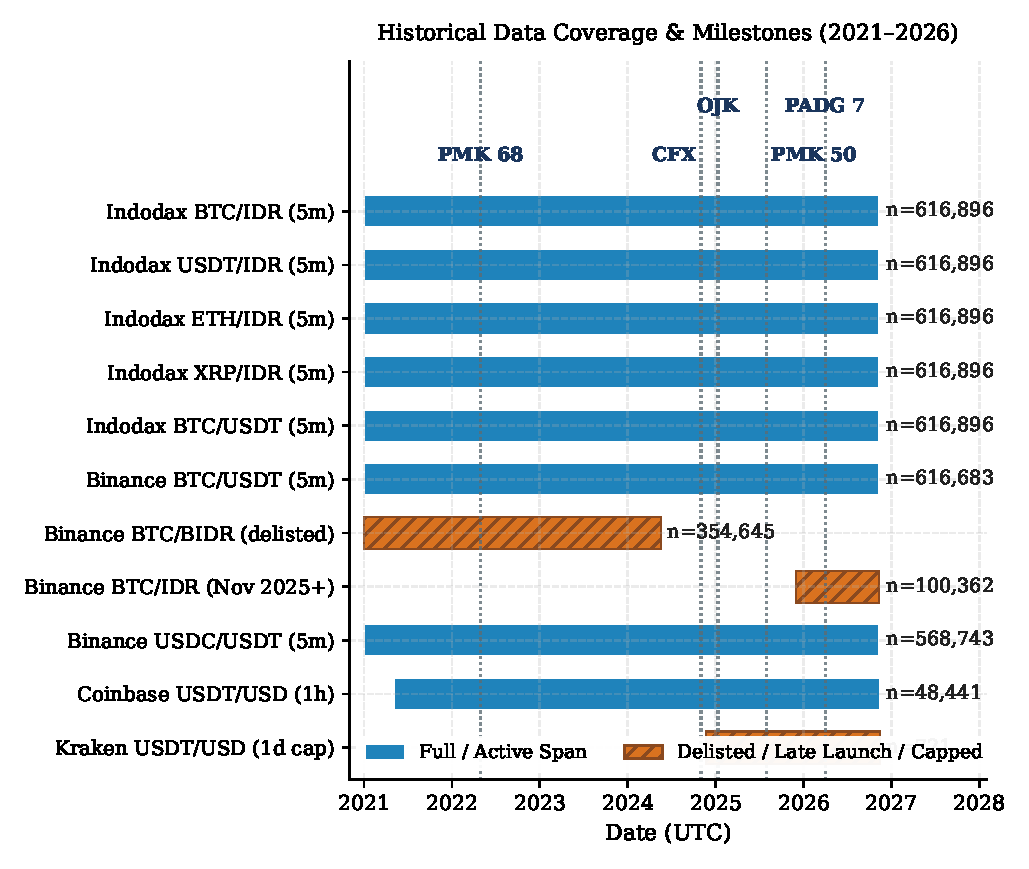
\includegraphics[width=\textwidth]{fig1_coverage_and_regimes.pdf}
  \caption{Historical instrument coverage matrix and Indonesian regulatory timeline (2021--2026).}
  \label{fig:coverage}
\end{figure}

\begin{figure}[htbp]
  \centering
  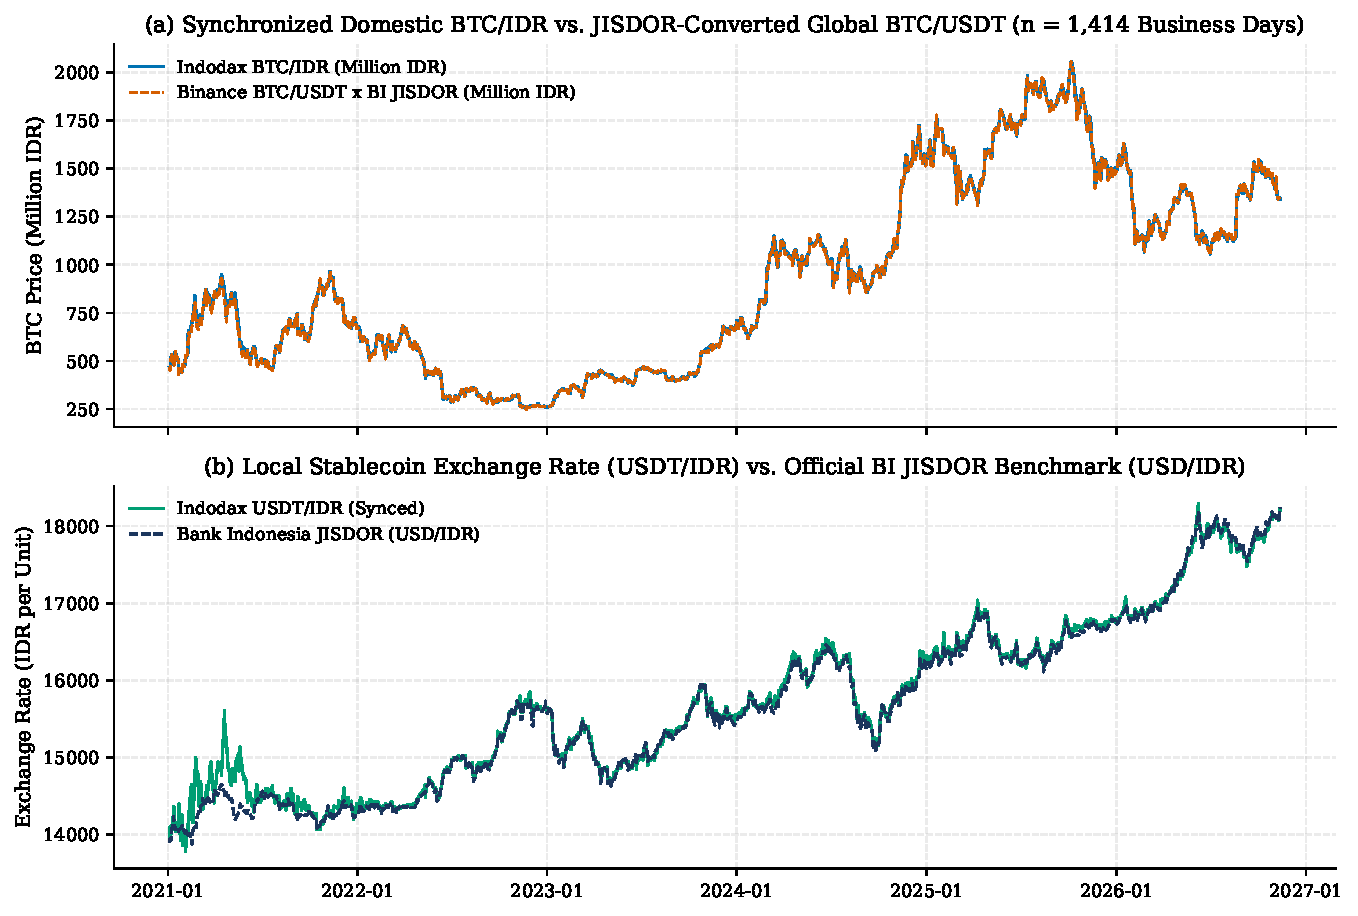
\includegraphics[width=\textwidth]{fig2_synchronized_prices.pdf}
  \caption{Synchronized domestic prices, JISDOR-converted global reference, and USDT/IDR vs.\ JISDOR (2021--2026).}
  \label{fig:prices}
\end{figure}

\section{Econometric methodology}
\label{sec:method}

\subsection{Three-leg basis and variance decomposition}
For cryptocurrency $X \in \{\mathrm{BTC}, \mathrm{ETH}, \mathrm{XRP}\}$ at synchronized time $t$, denote the domestic rupiah price on Indodax by $P_{X,t}^{IDR}$, the global Tether-quoted price on Binance by $P_{X,t}^{USDT}$, the domestic stablecoin exchange rate on Indodax by $U_t^{IDR/USDT}$, and the Bank Indonesia JISDOR USD/IDR fixing by $S_t^{IDR/USD}$. Defining log deviations in basis points ($\times 10^4$), we decompose the total basis relative to official USD/IDR into two economic legs:
\begin{align}
  B_t^{total} &= 10^4 \left( \ln P_{X,t}^{IDR} - \ln P_{X,t}^{USDT} - \ln S_t^{IDR/USD} \right), \label{eq:btot} \\
  B_t^{crypto} &= 10^4 \left( \ln P_{X,t}^{IDR} - \ln P_{X,t}^{USDT} - \ln U_t^{IDR/USDT} \right), \label{eq:bcry} \\
  B_t^{stablecoin\text{-}FX} &= 10^4 \left( \ln U_t^{IDR/USDT} - \ln S_t^{IDR/USD} \right), \label{eq:bsf}
\end{align}
so that $B_t^{total} \equiv B_t^{crypto} + B_t^{stablecoin\text{-}FX}$ holds identically at every date. Because USD and USDT can trade at a small spread, we separately track the USD/USDT peg wedge $W_t^{USD/USDT} = 10^4 \ln P_t^{USDT/USD}$ from Coinbase \texttt{USDT-USD} so that dollar-denominated pricing deviations are measured rather than assumed away. By bilinearity of covariance, total basis variance decomposes exactly as
\begin{equation}
  \mathrm{Var}(B_t^{total}) = \mathrm{Var}(B_t^{crypto}) + \mathrm{Var}(B_t^{stablecoin\text{-}FX}) + 2\,\mathrm{Cov}(B_t^{crypto}, B_t^{stablecoin\text{-}FX}).
  \label{eq:vardecomp}
\end{equation}
We verify numerically that discrepancy across the identity is below $10^{-10}\text{ bps}^2$. Because Equation~\eqref{eq:vardecomp} is an accounting identity, the variance shares describe which leg moves and do not identify a causal shock.

\subsection{Unit roots, cointegration tests, and residual bootstrap}
Because the rupiah exchange rate is $I(1)$, pairing rupiah-quoted bitcoin with unconverted USDT quotes inherits the exchange-rate unit root by construction; currency conversion is therefore necessary before testing cross-venue cointegration. After checking integration order with Augmented Dickey--Fuller (ADF), Phillips--Perron (PP) \citep{phillips1988testing}, KPSS \citep{kwiatkowski1992testing}, and single-break Zivot--Andrews \citep{zivot1992further} tests, we estimate three cointegration procedures (bootstrap $p$-values use $B = 9{,}999$ draws, so the smallest reportable value is $1/(B+1) = 0.0001$):
\begin{enumerate}
  \item \textbf{Engle--Granger (1987) two-step test:} Regresses $\ln P_{X,t}^{IDR} = a + \beta \ln P_{X,t}^{*} + e_t$ with OLS, testing $\hat{e}_t$ using MacKinnon (1996) residual response-surface critical values \citep{engle1987cointegration,mackinnon1996numerical}.
  \item \textbf{Fixed-$(1,-1)$ spread stationarity test:} Evaluates ADF and KPSS statistics directly on the imposed log spread $\ln P_{X,t}^{IDR} - \ln P_{X,t}^{*}$ without estimating $\beta$.
  \item \textbf{Johansen maximum likelihood with finite-sample corrections:} Evaluates Trace and Max-Eigenvalue statistics with a restricted constant in the cointegrating relation ($H_1^*(r)$, \texttt{det\_order=0}, $k_{ar\_diff}=1$ in daily baseline). Both Reinsel--Ahn (1992) statistic scaling $\frac{T - kp}{T}\lambda_{LR}$ and Cheung--Lai (1993) critical-value scaling $\frac{T}{T - kp} c_{\infty}$ are reported \citep{johansen1991estimation,reinsel1992vector,cheung1993finite}.
  \item \textbf{Null-imposed restricted VECM i.i.d.\ residual bootstrap ($B = 9,999$):} Following \citet{swensen2006bootstrap} and \citet{cavaliere2012bootstrap}, we estimate the restricted VAR in first differences under $H_0: \mathrm{rank}(\Pi) = 0$, center residuals, resample i.i.d.\ residual vectors recursively, and compute finite-sample $p$-values with Monte Carlo standard errors below $0.005$ at $p=0.5$. We validate empirical size and power in controlled Monte Carlo DGPs for $T \in \{25, 100, 500\}$.
\end{enumerate}

\subsection{VECM adjustment, price discovery, threshold models, and event windows}
For cointegrated pairs $Y_t = [\ln P_{X,t}^{IDR},\, \ln P_{X,t}^{*}]'$, we estimate the bivariate VECM:
\begin{equation}
  \Delta Y_t = \alpha \beta' Y_{t-1} + c + \sum_{j=1}^{p-1} \Gamma_j \Delta Y_{t-j} + u_t,
  \label{eq:vecm}
\end{equation}
reporting both ML standard errors and Newey--West HAC standard errors ($L=5$ daily, $L=12$ five-minute) for $\alpha_{local}$ and $\alpha_{global}$ \citep{newey1987simple}. Because JISDOR publishes only once per business day, the continuous 24/7 five-minute VECM converts global Binance \texttt{BTC/USDT} into rupiah using synchronous five-minute Indodax \texttt{USDT/IDR} candles ($\ln P_{BTC,t}^{*} = \ln P_{BTC,t}^{USDT} + \ln U_t^{IDR/USDT}$); both local prices therefore come from Indodax. Implied half-lives $-\ln(2)/\ln|1+\alpha_{local}|$ are reported in native sampling units (business days for daily panels, five-minute bars for intraday panels). Daily return pass-through regressions test whether global crypto returns, JISDOR changes, and \texttt{USDT/IDR}--JISDOR wedge changes transmit within-day or with a one-day lag.

Following \citet{hasbrouck1995one} and \citet{gonzalo1995estimation}, permanent-factor price discovery shares use Gonzalo--Granger weights $w_{global}^{GG} = |\alpha_{local}|/(|\alpha_{local}|+|\alpha_{global}|)$ and Cholesky-ordered Hasbrouck Information Share bounds $[IS_{low}, IS_{high}]$. Because daily contemporaneous residual correlation exceeds $0.99$, daily Hasbrouck bounds span nearly $[0,1]$ and are unidentifiable; we therefore examine Cholesky bounds only on the five-minute panel ($\rho_u = 0.671$).

To test transaction-cost band nonlinearity, we estimate a symmetric three-regime Band-TAR model on basis $B_t$ that nests the linear $\mathrm{AR}(p+1)$ model under $H_0$:
\begin{multline}
  \Delta B_t = c_{in}\mathbb{I}_{|B_{t-1}|\le\tau} + \rho_{in}(B_{t-1}\mathbb{I}_{|B_{t-1}|\le\tau}) + c_+\mathbb{I}_{B_{t-1}>\tau} + c_-\mathbb{I}_{B_{t-1}<-\tau} \\
  + \rho_{out}z_{out,t-1} + \sum_{j=1}^{p}\phi_j\Delta B_{t-j} + \varepsilon_t,
  \label{eq:tar}
\end{multline}
where $z_{out,t-1} = (B_{t-1} - \mathrm{sign}(B_{t-1})\tau)\mathbb{I}_{|B_{t-1}|>\tau}$. Grid search across the middle $70\%$ of $|B_t|$ yields the $\sup W(\tau)$ statistic, evaluated by linear-AR residual bootstrap \citep{hansen2002testing}. Regulatory event windows compare $\pm 30$ calendar days around ten documented institutional shocks using Welch $t$-tests and Mann--Whitney $U$ tests, with Holm adjustment across all 20 event $\times$ leg tests. As a robustness check against confounding market moves, we also estimate $\pm 30$-day OLS regressions with Newey--West HAC standard errors ($L=5$) controlling for daily global BTC log returns and daily JISDOR log returns.

\section{Empirical results}
\label{sec:results}

\subsection{Basis decomposition and variance shares}
Across the $n = 1,414$ synchronized Bank Indonesia JISDOR business days from January 4, 2021 through November 12, 2026, unadjusted Indonesian rupiah prices appear systematically elevated relative to global dollar-pegged benchmarks (Table~\ref{tab:descriptive}). The BTC total basis relative to BI JISDOR ($B_t^{total}$) averages $+29.94\text{ bps}$ ($95\%$ CI $[25.73, 34.15]\text{ bps}$), with a standard deviation of $80.80\text{ bps}$, a median of $+17.09\text{ bps}$ (IQR $57.44\text{ bps}$), and $66.27\%$ positive observations. Secondary and auxiliary assets mirror this pattern: $B_t^{total}$ averages $+30.22\text{ bps}$ (SD $83.52\text{ bps}$) for ETH and $+34.96\text{ bps}$ (SD $85.76\text{ bps}$) for XRP.

\begin{table}[htbp]
\centering
\caption{Descriptive Statistics of Basis Components and Exact Variance Decomposition (bps)}
\label{tab:descriptive}
\fontsize{6.8}{8}\selectfont\setlength{\tabcolsep}{2pt}
\begingroup
\begin{tabular}{@{}>{\raggedright\arraybackslash}p{2.5cm}rrrrrrr@{}}
\toprule
Sample / Basis Series & $N$ & Mean [95\% CI] & SD & Med. & IQR & $\%>0$ & $\le$ Taker \\
\midrule
BTC Primary: B\_total & 1,414 & 29.94 [25.73, 34.15] & 80.80 & 17.09 & 57.44 & 66.3\% & 82.2\% \\
BTC Primary: B\_crypto & 1,414 & -0.83 [-2.26, 0.60] & 27.44 & -0.79 & 27.29 & 48.6\% & 97.8\% \\
BTC Primary: B\_stablecoin\_FX & 1,414 & 30.77 [26.93, 34.61] & 73.66 & 18.77 & 38.43 & 75.0\% & 88.2\% \\
BTC Primary: W\_USD\_USDT & 1,331 & -1.13 [-1.57, -0.69] & 8.17 & 0.00 & 6.60 & 48.8\% & 99.9\% \\
ETH Primary: B\_total & 1,414 & 30.22 [25.87, 34.57] & 83.52 & 16.85 & 55.55 & 67.2\% & 82.7\% \\
ETH Primary: B\_crypto & 1,414 & -0.55 [-2.02, 0.92] & 28.16 & -1.26 & 27.26 & 47.2\% & 98.0\% \\
ETH Primary: B\_stablecoin\_FX & 1,414 & 30.77 [26.93, 34.61] & 73.66 & 18.77 & 38.43 & 75.0\% & 88.2\% \\
ETH Primary: W\_USD\_USDT & 1,331 & -1.13 [-1.57, -0.69] & 8.17 & 0.00 & 6.60 & 48.8\% & 99.9\% \\
XRP Primary: B\_total & 1,414 & 34.96 [30.49, 39.43] & 85.76 & 21.22 & 56.65 & 70.6\% & 81.5\% \\
XRP Primary: B\_crypto & 1,414 & 4.19 [2.34, 6.05] & 35.60 & 2.78 & 27.72 & 55.9\% & 97.0\% \\
XRP Primary: B\_stablecoin\_FX & 1,414 & 30.77 [26.93, 34.61] & 73.66 & 18.77 & 38.43 & 75.0\% & 88.2\% \\
XRP Primary: W\_USD\_USDT & 1,331 & -1.13 [-1.57, -0.69] & 8.17 & 0.00 & 6.60 & 48.8\% & 99.9\% \\
BTC All Calendar Days: B\_total & 2,136 & 33.11 [29.52, 36.69] & 84.62 & 20.83 & 62.25 & 67.2\% & 76.1\% \\
BTC Weekends Only: B\_total & 608 & 34.47 [27.61, 41.33] & 86.25 & 26.35 & 71.29 & 67.3\% & 69.2\% \\
BTC Weekends Only: B\_crypto & 608 & -1.70 [-3.92, 0.51] & 27.84 & -0.50 & 25.03 & 49.2\% & 98.4\% \\
\bottomrule
\end{tabular}\endgroup
\begin{minipage}{\textwidth}\footnotesize\vspace{3pt}
\emph{Exact Variance Identity (BTC, $n=1,414$):} $\mathrm{Var}(B^{total}) = 6529.03$ = $\mathrm{Var}(B^{crypto})\ (752.98,\ 11.53\%)$ + $\mathrm{Var}(B^{stable\text{-}FX})\ (5425.67,\ 83.10\%)$ + $2\mathrm{Cov}\,(350.38,\ 5.37\%)$. \emph{Dynamic Fee Band Containment (BTC $B^{crypto}$):} 64.57\% inside Route A maker band; 98.44\% inside Route A taker band; 98.94\% inside Route B taker band.
\end{minipage}
\end{table}


Separating currency conversion via local \texttt{USDT/IDR} accounts for the bulk of that premium. Once expressed in \texttt{USDT} using Indodax's synchronized \texttt{USDT/IDR} book, mean BTC pure-crypto basis ($B_t^{crypto}$) falls to $-0.83\text{ bps}$ ($95\%$ CI $[-2.26, +0.60]\text{ bps}$, SD $27.44\text{ bps}$, median $-0.79\text{ bps}$), which is statistically indistinguishable from zero at the $5\%$ level. ETH behaves identically ($B_t^{crypto}$ mean $-0.55\text{ bps}$, $95\%$ CI $[-2.02, +0.92]\text{ bps}$), while XRP shows a modest positive mean of $+4.19\text{ bps}$ (SD $35.60\text{ bps}$) alongside thinner domestic ask-to-bid symmetry ($17.31\text{ bps}$ snapshot round-trip spread at $\$1\text{k}$ on November 13, 2026). By contrast, the common domestic stablecoin--FX leg $B_t^{stablecoin\text{-}FX} = 10^4(\ln U_t^{IDR/USDT} - \ln S_t^{IDR/USD})$ averages $+30.77\text{ bps}$ ($95\%$ CI $[26.93, 34.61]\text{ bps}$, SD $73.66\text{ bps}$) and is positive on $75.04\%$ of business days. Over the $n = 1,331$ overlapping days after Coinbase \texttt{USDT-USD} launched on May 4, 2021, the external stablecoin peg wedge $W_t^{USD/USDT}$ averages $-1.13\text{ bps}$ (SD $8.17\text{ bps}$, median $0.00\text{ bps}$). Offshore USD-to-USDT drift therefore plays a secondary role except during transient stress events such as the $-171.46\text{ bps}$ low around March 2023.

\begin{figure}[htbp]
  \centering
  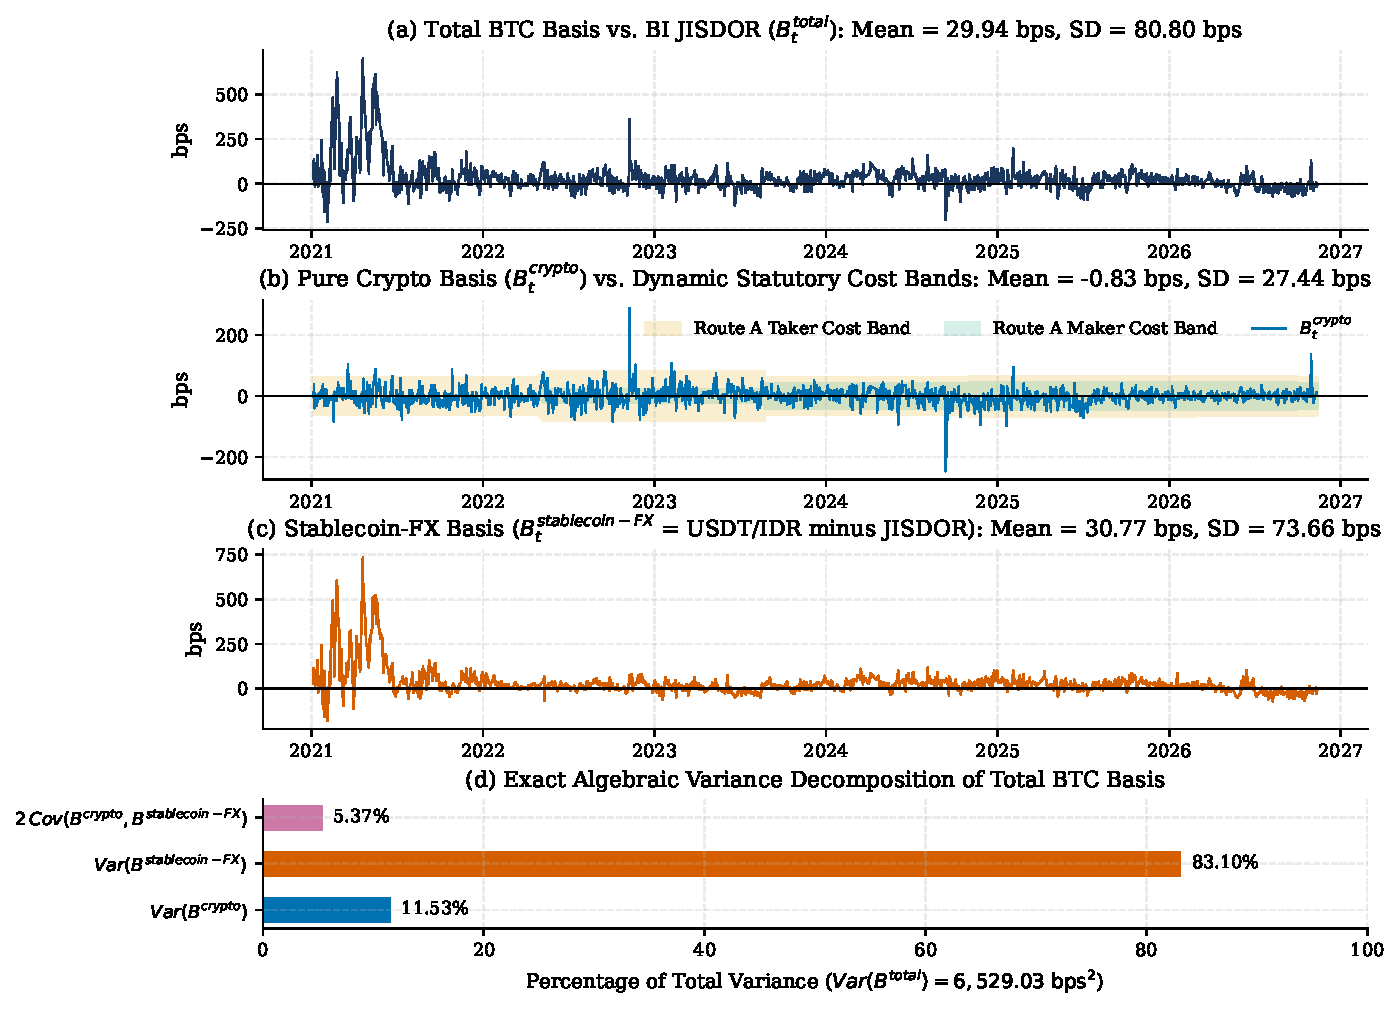
\includegraphics[width=\textwidth]{fig3_basis_decomposition.pdf}
  \caption{Two-leg basis decomposition for BTC from January 2021 through November 2026 ($n=1,414$ JISDOR business days), displaying $B_t^{total}$, $B_t^{crypto}$ inside dynamic domestic Route A taker cost bands, and the domestic stablecoin--FX basis $B_t^{stablecoin\text{-}FX}$.}
  \label{fig:decomp}
\end{figure}

The variance identity in Equation~\eqref{eq:vardecomp} shows which leg carries the movement in the total basis. For BTC, total basis variance $\mathrm{Var}(B_t^{total}) = 6,529.03\text{ bps}^2$ splits into $83.10\%$ for $\mathrm{Var}(B_t^{stablecoin\text{-}FX}) = 5,425.67\text{ bps}^2$, $11.53\%$ for $\mathrm{Var}(B_t^{crypto}) = 752.98\text{ bps}^2$, and $5.37\%$ for twice their covariance ($2\mathrm{Cov} = 350.38\text{ bps}^2$, contemporaneous correlation $0.0867$; identity discrepancy $9.1\times 10^{-13}\text{ bps}^2$). ETH and XRP show similar shares: $77.78\%$ versus $11.37\%$ for ETH ($10.85\%$ covariance), and $73.77\%$ versus $17.23\%$ for XRP ($9.00\%$ covariance). Figure~\ref{fig:decomp} plots the BTC basis series against time-varying domestic taker bands, and Figure~\ref{fig:dist} compares empirical distributions across all three cryptocurrencies. Evaluated date-by-date against regime-specific statutory taxes, CFX fees, and platform commissions (Section~\ref{sec:institutional}), $98.44\%$ of business-day BTC $B_t^{crypto}$ observations sit inside the dynamic two-leg domestic Route A taker band ($64.57\%$ inside the tighter maker band), and $98.94\%$ sit inside the cross-exchange Route B three-leg taker band. Against the fixed sample-average Route A taker threshold ($66.45\text{ bps}$, reported in the final column of Table~\ref{tab:descriptive}), containment is $97.81\%$. Across extreme interpretations of the partially verified May 2022--October 2024 Indodax fee transition ($61.0\text{ bps}$ versus $81.0\text{ bps}$ taker throughout), dynamic Route A containment stays within $[97.52\%, 98.51\%]$. Because $B_t^{crypto}$ has a standard deviation of $27.44\text{ bps}$, this high containment rate follows mechanically from its narrow dispersion relative to the $60.0$--$81.0\text{ bps}$ taker band and does not by itself prove the absence of exploitable intraday arbitrage.

\begin{figure}[htbp]
  \centering
  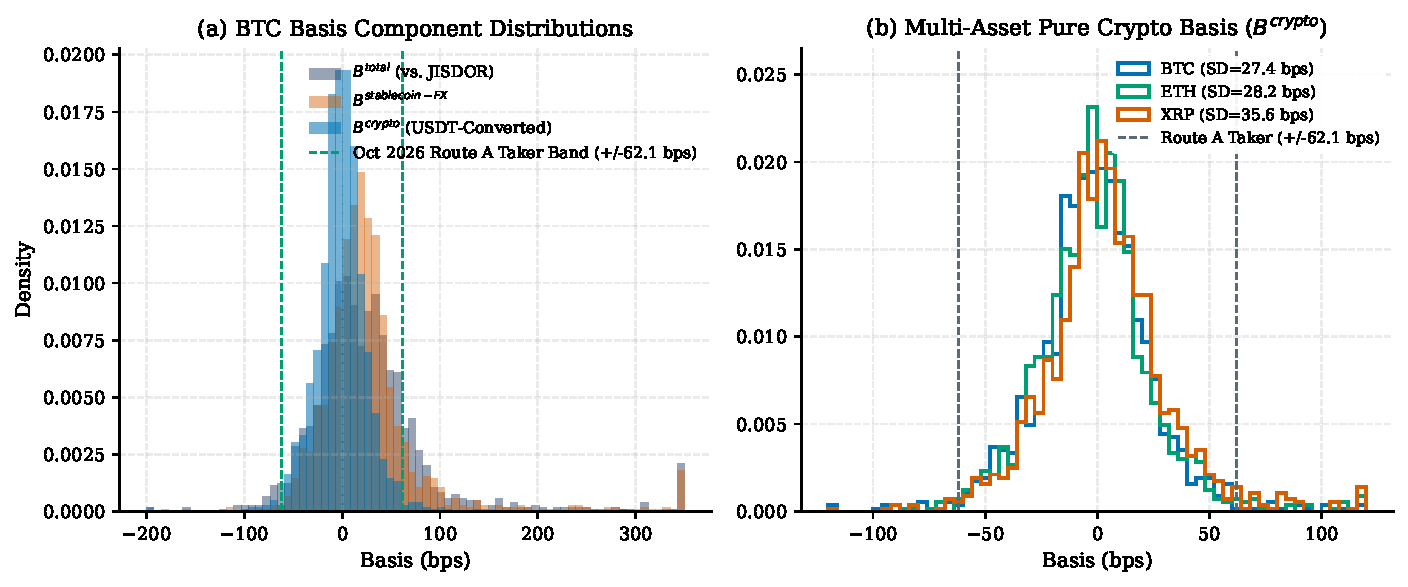
\includegraphics[width=\textwidth]{fig4_basis_distributions.pdf}
  \caption{Empirical basis distributions ($B_t^{total}$, $B_t^{crypto}$, $B_t^{stablecoin\text{-}FX}$) and multi-asset pure crypto basis ($B_t^{crypto}$) across BTC, ETH, and XRP. Extreme observations are winsorized at $[-180, 320]\text{ bps}$ in Panel~(a) and $[-120, 120]\text{ bps}$ in Panel~(b) for display.}
  \label{fig:dist}
\end{figure}

\subsection{Unit-root properties and cointegration rank}
Table~\ref{tab:unit_roots} reports ADF, Phillips--Perron, KPSS, and Zivot--Andrews single-break tests across all price levels, first differences, and basis series. Every log asset price ($\ln P_{t}^{IDR}$, $\ln P_{t}^{USDT}$) and FX benchmark ($\ln U_t^{IDR/USDT}$, $\ln S_t^{IDR/USD}$) fails to reject a unit root under ADF and PP ($p \ge 0.626$ with constant; Zivot--Andrews statistics $-3.13$ to $-3.78$ versus the $-4.80$ critical value) while rejecting KPSS stationarity ($p = 0.01$), consistent with $I(1)$ log levels and $I(0)$ first differences ($p < 0.0001$). For basis spreads, $B_t^{crypto}$ rejects a unit root ($ADF = -10.62$, $p < 0.0001$ for BTC; $-10.59$ for ETH; $-9.58$ for XRP) and fails to reject KPSS constant-mean stationarity for BTC ($\eta_\mu = 0.380$, $p = 0.086$) and ETH ($\eta_\mu = 0.383$, $p = 0.085$). By contrast, $B_t^{total}$ and $B_t^{stablecoin\text{-}FX}$ reject unit roots under ADF and PP ($p < 0.0001$) yet reject KPSS constant-mean stationarity ($\eta_\mu = 1.27$--$1.58$, $p = 0.01$). That divergence indicates level shifts in onshore stablecoin premia over 2021--2026 rather than a random walk.

\begin{table}[htbp]
\centering
\caption{Unit-root and stationarity tests (2021--2026 synchronized business-day panel)}
\label{tab:unit_roots}
\fontsize{6.6}{7.8}\selectfont\setlength{\tabcolsep}{2pt}
\begingroup
\begin{tabular}{@{}>{\raggedright\arraybackslash}p{3.4cm}rrrrrr@{}}
\toprule
Series & $N$ & ADF (Const.) & $p$-val & PP ($Z_t$) & KPSS ($\eta_\mu$) & Zivot--Andrews \\
\midrule
BTC ln P\_IDR & 1,414 & -1.072 & 0.7262 & -1.185 & 3.483 & -3.123 \\
BTC d(ln P\_IDR) & 1,413 & -15.251 & $<$0.0001 & -36.442 & 0.107 & -15.510 \\
BTC ln P\_USDT & 1,414 & -1.237 & 0.6574 & -1.317 & 3.059 & -3.163 \\
BTC d(ln P\_USDT) & 1,413 & -37.176 & $<$0.0001 & -37.226 & 0.104 & -37.349 \\
Indodax ln U\_IDR (USDT/IDR) & 1,414 & -0.356 & 0.9171 & -0.622 & 4.998 & -3.680 \\
Indodax d(ln U\_IDR) & 1,413 & -12.156 & $<$0.0001 & -39.452 & 0.050 & -13.893 \\
BI JISDOR ln S\_FX & 1,414 & -0.268 & 0.9300 & -0.385 & 5.044 & -3.782 \\
BI JISDOR d(ln S\_FX) & 1,413 & -13.093 & $<$0.0001 & -34.045 & 0.060 & -13.226 \\
BTC B\_total (bps) & 1,414 & -5.348 & $<$0.0001 & -16.339 & 1.316 & -7.319 \\
BTC B\_crypto (bps) & 1,414 & -10.280 & $<$0.0001 & -31.971 & 0.383 & -11.028 \\
BTC B\_stablecoin\_FX (bps) & 1,414 & -4.878 & $<$0.0001 & -12.102 & 1.271 & -7.402 \\
ETH B\_total (bps) & 1,414 & -5.290 & $<$0.0001 & -16.947 & 1.295 & -7.389 \\
ETH B\_crypto (bps) & 1,414 & -10.718 & $<$0.0001 & -31.316 & 0.418 & -11.273 \\
XRP B\_total (bps) & 1,414 & -6.186 & $<$0.0001 & -19.444 & 1.648 & -7.527 \\
XRP B\_crypto (bps) & 1,414 & -32.630 & $<$0.0001 & -34.761 & 2.465 & -33.617 \\
\bottomrule
\end{tabular}\endgroup
\begin{minipage}{\textwidth}\footnotesize\vspace{3pt}
\emph{Notes:} 5\% critical values: ADF constant $-2.864$, KPSS constant $0.463$ ($H_0$: stationarity), Zivot--Andrews single-break $-4.80$. All log price levels and FX series are $I(1)$; first differences and all basis spreads reject a unit root at $p < 0.0001$.
\end{minipage}
\end{table}


Table~\ref{tab:cointegration} demonstrates how omitting FX conversion reverses cointegration conclusions. Pairing Indodax \texttt{BTC/IDR} with unconverted Binance \texttt{BTC/USDT} fails every test for long-run equilibrium: Engle--Granger yields $t = -1.10$ ($p = 0.881$), Fixed-$(1,-1)$ ADF yields $-0.40$ ($p = 0.909$), Reinsel--Ahn Johansen trace is $6.33$ (far below both the $15.49$ asymptotic and $15.54$ Cheung--Lai $5\%$ critical values), and the $B = 9,999$ null-imposed restricted-VECM block-wild bootstrap ($b = 6$) returns $p_{boot} = 0.8584$. Unadjusted ETH ($\text{Trace}_{RA} = 11.20$, $p_{boot} = 0.4774$) and XRP ($\text{Trace}_{RA} = 8.38$, $p_{boot} = 0.7734$) fail identically.

\begin{table}[htbp]
\centering
\caption{Engle--Granger, Fixed-$(1,-1)$, Johansen (Reinsel--Ahn), and Bootstrap Cointegration Tests ($B=9,999$)}
\label{tab:cointegration}
\fontsize{6.3}{7.5}\selectfont\setlength{\tabcolsep}{2pt}
\begingroup
\begin{tabular}{@{}>{\raggedright\arraybackslash}p{2.5cm}rrrrrrr@{}}
\toprule
Specification & $T_{eff}$ & EG $\hat{\beta}$ & EG $t$ & Fixed ADF & Trace (RA) & MaxEig (RA) & Boot $p$ \\
\midrule
BTC Unadjusted & 1,412 & 1.0702 & -1.10 & -0.40 & 6.33 & 5.75 & 0.7314 \\
BTC JISDOR & 1,412 & 0.9993 & -4.42 & -5.37 & 151.72 & 150.32 & $\le$0.0001 \\
BTC USDT & 1,412 & 0.9994 & -10.97 & -10.62 & 513.96 & 512.73 & $\le$0.0001 \\
BTC SpotFX & 1,249 & 1.0003 & -4.81 & -6.73 & 151.09 & 149.66 & $\le$0.0001 \\
USDT IDR vs JISDOR & 1,412 & 0.9673 & -4.65 & -4.89 & 102.68 & 102.55 & $\le$0.0001 \\
ETH Unadjusted & 1,412 & 1.0161 & -0.60 & -0.44 & 11.20 & 9.11 & 0.2821 \\
ETH JISDOR & 1,412 & 0.9998 & -4.28 & -5.27 & 141.46 & 132.40 & $\le$0.0001 \\
ETH USDT & 1,412 & 0.9996 & -10.53 & -10.59 & 511.04 & 502.18 & $\le$0.0001 \\
XRP Unadjusted & 1,412 & 1.0523 & -0.86 & -0.40 & 8.38 & 6.09 & 0.5280 \\
XRP JISDOR & 1,412 & 0.9994 & -4.14 & -5.16 & 131.12 & 126.46 & $\le$0.0001 \\
XRP USDT & 1,412 & 0.9993 & -9.94 & -9.58 & 492.91 & 488.34 & $\le$0.0001 \\
\midrule
\multicolumn{8}{@{}l}{\textbf{Monte Carlo Validation of Null-Imposed VECM Bootstrap Size \& Power ($n_{MC}=150$, $B=299$):}} \\
DGP $T=25$, $r=0$ (Size) & \multicolumn{2}{r}{Asymp: 16.7\%} & \multicolumn{2}{r}{RA: 6.7\%} & \multicolumn{3}{r}{Bootstrap: 3.3\%} \\
DGP $T=25$, $r=1$ (Power) & \multicolumn{2}{r}{Asymp: 37.3\%} & \multicolumn{2}{r}{RA: 14.0\%} & \multicolumn{3}{r}{Bootstrap: 10.0\%} \\
DGP $T=100$, $r=0$ (Size) & \multicolumn{2}{r}{Asymp: 11.3\%} & \multicolumn{2}{r}{RA: 8.7\%} & \multicolumn{3}{r}{Bootstrap: 4.0\%} \\
DGP $T=100$, $r=1$ (Power) & \multicolumn{2}{r}{Asymp: 90.7\%} & \multicolumn{2}{r}{RA: 86.7\%} & \multicolumn{3}{r}{Bootstrap: 76.0\%} \\
DGP $T=500$, $r=0$ (Size) & \multicolumn{2}{r}{Asymp: 12.0\%} & \multicolumn{2}{r}{RA: 11.3\%} & \multicolumn{3}{r}{Bootstrap: 6.0\%} \\
DGP $T=500$, $r=1$ (Power) & \multicolumn{2}{r}{Asymp: 100.0\%} & \multicolumn{2}{r}{RA: 100.0\%} & \multicolumn{3}{r}{Bootstrap: 100.0\%} \\
\bottomrule
\end{tabular}\endgroup
\begin{minipage}{\textwidth}\footnotesize\vspace{3pt}
\emph{Notes:} 5\% critical values: Engle--Granger $-3.340$; Fixed-$(1,-1)$ ADF $-2.864$; Johansen asymptotic Trace $15.49$, MaxEig $14.26$ (Cheung--Lai 5\% CV at $T_{eff}=1,412$: Trace $15.54$, MaxEig $14.30$). Null-imposed restricted-VECM i.i.d. residual bootstrap uses $B=9,999$ replications.
\end{minipage}
\end{table}


Introducing synchronized currency conversion overturns those null results cleanly. Converting global \texttt{BTC/USDT} at BI JISDOR raises the Reinsel--Ahn trace statistic from $6.33$ to $151.72$ ($p_{boot} = 0.0001$, Engle--Granger $\hat{\beta} = 0.9993$, $t = -4.42$, $p = 0.0016$, Fixed-$(1,-1)$ ADF $-5.37$, $p < 0.0001$). Converting instead via domestic \texttt{USDT/IDR} raises the trace statistic further to $513.96$ ($p_{boot} = 0.0001$, Fixed ADF $-10.62$) because local crypto pairs and the domestic stablecoin leg move tightly together. Both ETH ($\text{Trace}_{RA} = 141.46$ JISDOR, $511.04$ USDT, $p_{boot} = 0.0001$) and XRP ($\text{Trace}_{RA} = 131.12$ JISDOR, $492.91$ USDT, $p_{boot} = 0.0001$) yield identical rank $r=1$ findings, and domestic \texttt{USDT/IDR} itself is cointegrated with BI JISDOR ($\text{Trace}_{RA} = 102.68$, block-wild $p_{boot} = 0.0005$ against a $5\%$ bootstrap critical value of $46.65$, $\hat{\beta}_{EG} = 0.9673$). No rank-$2$ trace test exceeds its $5\%$ critical value for BTC ($1.41$ and $1.24$ versus $3.84$), which is consistent with a single common stochastic trend. Appendix Table~\ref{tab:boot_mc} validates the block-wild bootstrap across $n_{MC} = 1,000$ replications under GARCH(1,1) and AR(1) innovations. Figure~\ref{fig:rolling} illustrates 60-business-day rolling basis averages, rolling volatility (standard deviation), and rolling cross-leg correlations through 2021--2026.

\begin{figure}[htbp]
  \centering
  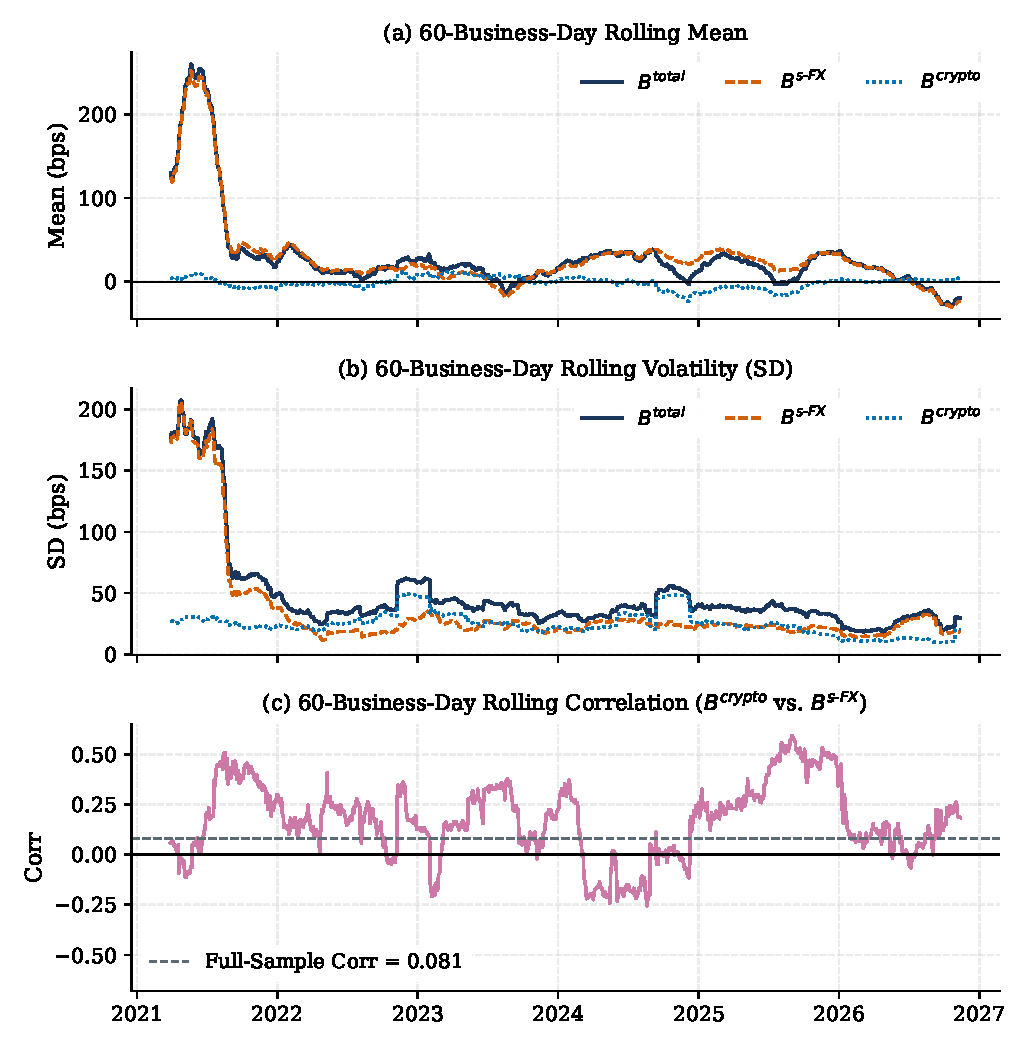
\includegraphics[width=\textwidth]{fig5_rolling_dynamics_and_corr.pdf}
  \caption{Rolling 60-business-day BTC basis means, volatility (SD), and cross-leg correlation between $B_t^{crypto}$ and $B_t^{stablecoin\text{-}FX}$ (2021--2026).}
  \label{fig:rolling}
\end{figure}

\subsection{Error-correction speeds, three-variable intraday price discovery, and threshold dynamics}
Table~\ref{tab:vecm_ecm} reports VECM estimates (Panel A daily business-day bivariate systems; Panel B five-minute 24/7 three-variable BTC systems), and Figure~\ref{fig:ec} contrasts Johansen trace statistics and daily adjustment speeds. On the synchronized daily panel ($T_{eff} = 1,412$, one lagged difference, HAC $L = 5$), Indodax BTC absorbs the error-correction burden against JISDOR-converted global BTC ($\hat{\alpha}_{local} = -0.398$, HAC SE $0.165$, $p = 0.0158$), while we fail to reject weak exogeneity for global BTC ($\hat{\alpha}_{global} = -0.213$, HAC SE $0.195$, $p = 0.2728$; LR weak-exogeneity $p = 0.092$). Accounting for full-VECM companion dynamics rather than $\alpha_{local}$ alone yields a native companion-root half-life of $3.66$ business days ($|\lambda_{\max}| = 0.8275$). Converting global BTC at domestic \texttt{USDT/IDR} increases the local adjustment speed ($\hat{\alpha}_{local} = -0.884$, HAC $p = 0.0231$, full-system half-life $0.56$ business days). For ETH and XRP, daily $\hat{\alpha}_{local}$ estimates carry the expected negative sign ($-0.193$ to $-0.775$) but are statistically insignificant under HAC standard errors ($p = 0.148$ to $0.402$) due to noisy daily aggregation. In both daily BTC systems, cross-market innovations are nearly collinear ($\rho_u = 0.991$ and $0.997$), so daily Cholesky Hasbrouck bounds span nearly $[0, 1]$ and are uninformative. In the Indodax \texttt{USDT/IDR}--JISDOR currency system ($\rho_u = 0.566$), we fail to reject weak exogeneity for JISDOR ($p = 0.205$), while Indodax \texttt{USDT/IDR} error-corrects ($\hat{\alpha}_{local} = -0.142$, HAC $p < 0.0001$, full-system half-life $4.28$ business days).

\begin{table}[htbp]
\centering
\caption{VECM Error Correction, Price Discovery, Band-TAR, and Return Pass-Through}
\label{tab:vecm_ecm}
\fontsize{6.3}{7.5}\selectfont\setlength{\tabcolsep}{2pt}
\begingroup
\begin{tabular}{@{}>{\raggedright\arraybackslash}p{2.5cm}rrrrrrr@{}}
\toprule
\multicolumn{8}{@{}l}{\textbf{Panel A: Daily Bivariate VECM Estimates (Native Day Units, HAC $L=5$)}} \\
System & $T_{eff}$ & $\hat{\alpha}_{local}$ (SE) & $p_{loc}$ & $\hat{\alpha}_{glob}$ & $p_{glob}$ & HL (d) & GG $w_g$ \\
\midrule
BTC vs JISDOR-Global & 1,412 & -0.398 (0.165) & 0.0158 & -0.213 & 0.2728 & 1.36 & 65.1\% \\
BTC vs USDT-Global & 1,412 & -0.884 (0.389) & 0.0231 & -0.105 & 0.7921 & 0.32 & 89.4\% \\
Indodax USDT/IDR vs BI JISDOR & 1,412 & -0.142 (0.033) & $<$0.0001 & 0.016 & 0.2050 & 4.53 & 89.6\% \\
ETH vs JISDOR-Global & 1,412 & -0.193 (0.230) & 0.4016 & -0.003 & 0.9892 & 3.23 & 98.3\% \\
ETH vs USDT-Global & 1,412 & -0.775 (0.536) & 0.1484 & 0.000 & 0.9994 & 0.46 & 99.9\% \\
XRP vs JISDOR-Global & 1,412 & -0.361 (0.287) & 0.2087 & -0.159 & 0.6073 & 1.55 & 69.4\% \\
XRP vs USDT-Global & 1,412 & -0.530 (0.574) & 0.3556 & 0.284 & 0.6302 & 0.92 & 65.1\% \\
\midrule
\multicolumn{8}{@{}l}{\textbf{Panel B: 5-Minute 24/7 BTC VECM \& Band-TAR Diagnostics (Native 5m Bar Units)}} \\
5m All Bars ($k=5$, HAC $L=12$) & 616,677 & -0.0468 (0.0024) & $<$0.0001 & 0.0095 & $<$0.0001 & 14.45 & 83.2\% \\
5m Active-Vol Bars ($k=5$) & 605,150 & -0.0608 (0.0019) & $<$0.0001 & 0.0120 & $<$0.0001 & 11.04 & 83.6\% \\
\midrule
\multicolumn{8}{@{}l}{\textbf{Panel C: Daily Log-Return Pass-Through $\Delta\ln P_t^{IDR} = c + \beta_1 \Delta\ln P_t^{USDT} + \beta_2 \Delta\ln S_t^{FX} + \beta_3 \Delta(B_t^{s\text{-}FX})$}} \\
Asset & $N$ & $\hat{\beta}_{crypto}$ (SE) & $\hat{\beta}_{FX}$ (SE) & $\hat{\beta}_{s\text{-}FX}$ (SE) & Adj. $R^2$ & $\hat{\beta}_{t-1}^{cry}$ & $p_{t-1}$ \\
\midrule
BTC & 1,412 & 0.9684 (0.0035) & 0.9322 (0.0273) & 0.9612 (0.0341) & 0.9906 & 0.0212 & $<$0.0001 \\
ETH & 1,412 & 0.9757 (0.0030) & 0.9713 (0.0263) & 1.0289 (0.0311) & 0.9943 & 0.0158 & $<$0.0001 \\
XRP & 1,412 & 0.9834 (0.0029) & 0.9960 (0.0353) & 0.9967 (0.0394) & 0.9940 & 0.0116 & $<$0.0001 \\
\bottomrule
\end{tabular}\endgroup
\begin{minipage}{\textwidth}\footnotesize\vspace{3pt}
\emph{Notes:} 5m Active Hasbrouck Information Share (Global): [44.3\%, 98.9\%] (midpoint 71.6\%, $\rho_u=0.671$); daily BTC $\rho_u=0.991$. Band-TAR daily $B^{crypto}$: $\hat{\tau}=28.81$ bps, $\sup W=7.05$ ($p=0.392$); 5m Active ($n=25k$): $\hat{\tau}=17.81$ bps, $\sup W=362.40$ ($p=0.0033$, $\rho_{in}=-0.160$, $\rho_{out}=-0.012$).
\end{minipage}
\end{table}


\begin{figure}[htbp]
  \centering
  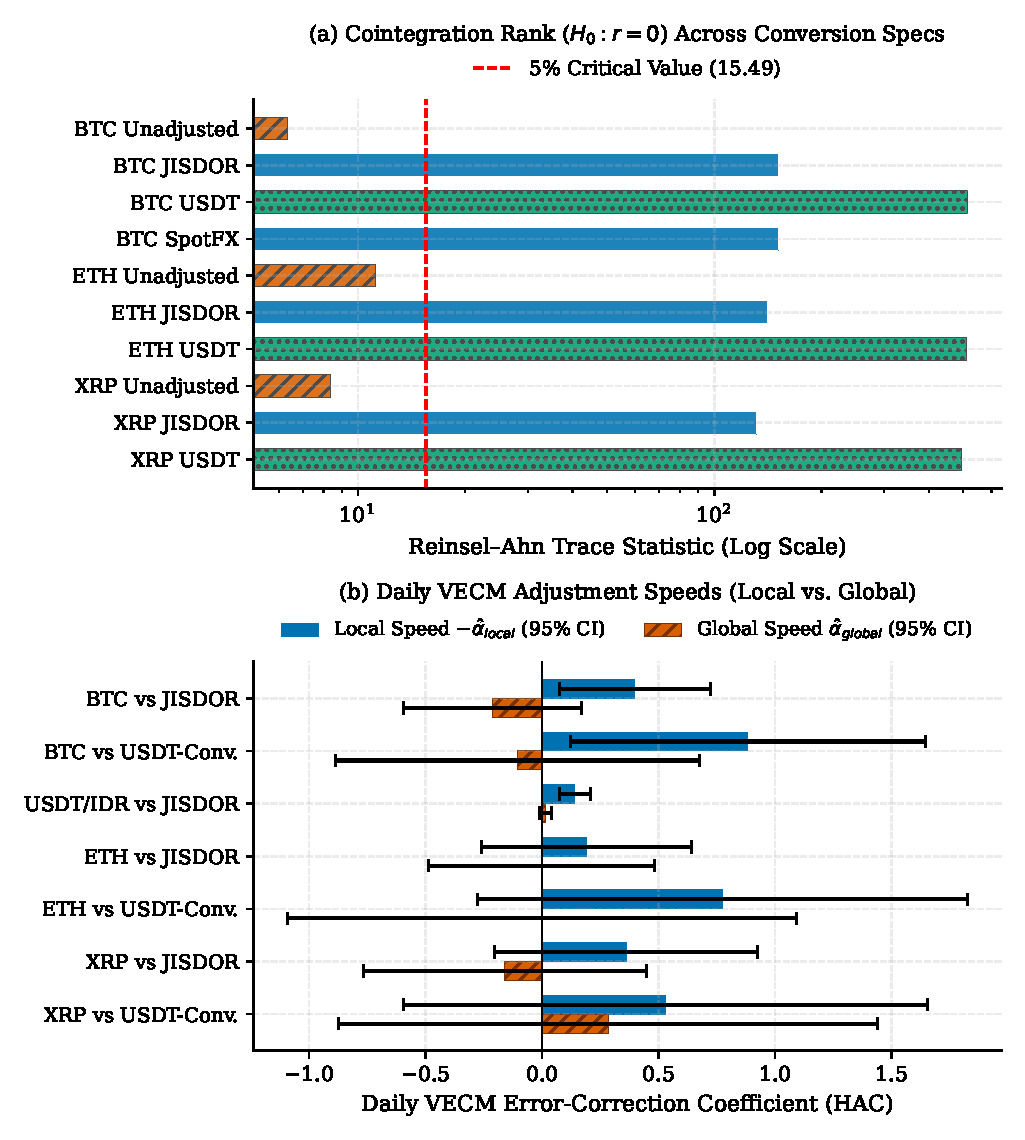
\includegraphics[width=\textwidth]{fig6_cointegration_and_ec.pdf}
  \caption{Unadjusted versus FX-converted Johansen trace statistics (Reinsel--Ahn, Panel~a) and daily VECM error-correction speeds with HAC 95\% confidence intervals (Panel~b).}
  \label{fig:ec}
\end{figure}

To analyze intraday price discovery without embedding domestic \texttt{USDT/IDR} into a synthetic global BTC price, Panel~B of Table~\ref{tab:vecm_ecm} estimates a three-variable five-minute VECM on the regular clock-time grid ($T_{eff} = 616,677$ equally spaced five-minute bars, five lagged differences, HAC $L = 12$) using $Y_t = [\ln P_{BTC,t}^{IDR},\, \ln P_{BTC,t}^{USDT},\, \ln U_t^{IDR/USDT}]'$. Both asymptotic Johansen rank tests ($\text{Trace}_{r=0} = 9,125.5$ vs.\ $5\%$ CV $29.80$; $\text{Trace}_{r\le 1} = 11.10$ vs.\ $15.49$) and the dependence-preserving block-wild bootstrap ($B = 499$, block length $b = 28$; $\text{Trace}_{r=0}$ bootstrap $p = 0.0020$ against $5\%$ bootstrap CV $56.19$) reject zero cointegration and support rank $r = 1$ with cointegrating vector $\hat{\beta} = [1.0000,\,-0.9994,\,-1.0045]'$.

Separating the three markets yields clear adjustment asymmetries, though cross-market price leadership remains bounded rather than uniquely identified. We fail to reject weak exogeneity for global Binance \texttt{BTC/USDT} ($\hat{\alpha}_{BTC/USDT} = +0.0011$, HAC SE $0.0014$, $p = 0.4179$), which accounts for $2.0\%$ of total error-correction adjustment. By contrast, Indodax \texttt{BTC/IDR} bears $80.0\%$ of error correction ($\hat{\alpha}_{BTC/IDR} = -0.0445$, HAC SE $0.0023$, $p < 0.0001$) and Indodax \texttt{USDT/IDR} bears the remaining $18.0\%$ ($\hat{\alpha}_{USDT/IDR} = +0.0100$, HAC SE $0.0007$, $p < 0.0001$). Inspecting the full companion matrix eigenvalues reveals a sharp spectral gap: the largest non-unit eigenvalue modulus is $|\lambda_{\max}| = 0.9728$ (implying a slowest-mode half-life of $25.08$ five-minute bars, compared with the scalar $1 + \beta'\alpha$ benchmark of $12.09$ bars), whereas the next-largest non-unit moduli are $\{0.5786, 0.5786\}$ (half-life $1.27$ bars), confirming that $|\lambda_{\max}| = 0.9728$ isolates the persistent error-correction mode rather than transient short-run lag dynamics. Across all six Cholesky orderings of $\Psi(1)$, Hasbrouck Information Share bounds for the permanent component of Indodax \texttt{BTC/IDR} span $[42.6\%, 99.0\%]$ for Binance \texttt{BTC/USDT}, $[1.0\%, 54.8\%]$ for Indodax \texttt{BTC/IDR}, and $[0.0\%, 3.0\%]$ for Indodax \texttt{USDT/IDR}; because the Binance and Indodax \texttt{BTC/IDR} bounds overlap, Hasbrouck shares indicate substantial global information transmission without uniquely isolating a single price leader.

Two sensitivity checks confirm the stability of this pattern. First, dropping the 11,533 zero-volume bars yields an irregularly spaced active-volume subsample ($T_{eff} = 605,150$) with similar adjustment shares ($80.3\%$ Indodax \texttt{BTC/IDR}, $1.3\%$ Binance \texttt{BTC/USDT}, $18.4\%$ Indodax \texttt{USDT/IDR}) but a faster active-bar companion half-life ($19.42$ active observations; scalar $9.25$), which should not be interpreted in regular five-minute clock units. Second, replacing Indodax \texttt{USDT/IDR} with Binance's native \texttt{USDT/IDR} over the 349-day overlap ($T_{eff} = 100,356$ regular bars) preserves non-rejection of weak exogeneity for global Binance \texttt{BTC/USDT} ($\hat{\alpha} = +0.0002$, HAC $p = 0.8580$; Hasbrouck IS $[25.0\%, 93.8\%]$), while Indodax \texttt{BTC/IDR} ($\hat{\alpha} = -0.0164$, HAC $p = 0.0001$, $48.0\%$ share) and Binance's thinner \texttt{USDT/IDR} book ($\hat{\alpha} = +0.0175$, HAC $p = 0.1833$, $51.3\%$ share) split domestic adjustment (companion half-life $22.17$ bars). Daily VECM residuals for \texttt{USDT/IDR}--JISDOR and five-minute BTC equations exhibit serial correlation and ARCH clustering ($\text{LB } p < 0.001$, $\text{ARCH } p < 0.001$), which motivates HAC standard errors for adjustment inference and our block-wild bootstrap for cointegration rank tests.

Threshold Band-TAR tests qualify the linear error-correction results across regimes. On daily $B_t^{crypto}$, the estimated threshold is $\hat{\tau} = 28.81\text{ bps}$, and the wild-bootstrap linearity test fails to reject linearity ($\sup W = 7.05$, $B = 499$, $p = 0.392$). By contrast, daily $B_t^{total}$ rejects linearity ($\hat{\tau} = 69.22\text{ bps}$, $\sup W = 72.92$, $p = 0.002$) with slower outer adjustment ($\hat{\rho}_{out} = -0.051$ vs.\ $\hat{\rho}_{in} = -0.390$, $13.25$-day outer half-life). At five-minute frequency, active-bar Band-TAR behavior varies by period: in an early 2022--2023 subsample ($n = 25,000$ active bars), linearity is rejected ($\hat{\tau} = 44.36\text{ bps}$, $\sup W = 202.38$, $B = 299$, $p = 0.0033$) with faster outer-band adjustment ($\hat{\rho}_{out} = -0.302$ vs.\ $\hat{\rho}_{in} = -0.080$, outer half-life $1.93$ bars), whereas in the recent 2026 subsample ($n = 25,000$ active bars), linearity is rejected ($\hat{\tau} = 17.81\text{ bps}$, $\sup W = 362.40$, $p = 0.0033$) with slower outer adjustment ($\hat{\rho}_{out} = -0.0115$ vs.\ $\hat{\rho}_{in} = -0.160$). Finally, in daily return dynamics ($n = 1,412$), contemporaneous regressions of $\Delta \ln P_t^{IDR}$ on $\Delta \ln P_t^{USDT}$, $\Delta \ln S_t^{FX}$, and $\Delta(\ln U_t - \ln S_t)$ hold nearly by accounting identity (Adjusted $R^2 > 0.99$); the informative non-mechanical test is the one-day lagged global crypto return, which carries a small positive catch-up coefficient of $+0.0212$ for BTC ($+0.0158$ ETH, $+0.0116$ XRP, all HAC $p < 0.0001$).

\subsection{Regulatory regimes, controlled event windows, and snapshot execution costs}
Table~\ref{tab:events} and Figure~\ref{fig:events} evaluate $\pm 30$-calendar-day event windows across ten regulatory, tax, and exchange-structure milestones from May 2022 through October 2026 \citep{pmk68_2022,binance_bidr_2024,indodax_events_2026,perba9_2024,pojk27_2024,pmk50_2025,cfx_seb001_2026,bi_padg072026}. Our primary inference uses $\pm 30$-day OLS regressions controlling for daily global BTC and JISDOR log returns with Newey--West HAC standard errors ($L=5$), with Holm multiple-testing adjustment applied across the 20-test BTC event $\times$ leg family. Because three event pairs overlap within $\pm 30$ calendar days and the October 31, 2026 maintenance event has only 12 post-event calendar days before our November 12, 2026 cutoff, Table~\ref{tab:events} also reports a simultaneous full-sample regression using non-overlapping $\pm 15$-day pre/post indicators.

\begin{table}[htbp]
\centering
\caption{30-Calendar-Day Pre/Post Institutional and Regulatory Event Windows (BTC Basis, bps)}
\label{tab:events}
\fontsize{6.3}{7.5}\selectfont\setlength{\tabcolsep}{2pt}
\begingroup
\begin{tabular}{@{}l>{\raggedright\arraybackslash}p{2.3cm}rrrrrr@{}}
\toprule
Date & Event & $\Delta\bar{B}^{cry}$ & $p_W$ ($p_{\text{Holm}}$) & $p_{\text{MW}}$ & $\Delta\bar{B}^{s\text{-}FX}$ & $p_W$ ($p_{\text{Holm}}$) & $p_{\text{MW}}$ \\
\midrule
2022-05-01 & PMK 68/2022 Tax & 13.23 & 0.293 (1.000) & 0.222 & 7.05 & 0.419 (1.000) & 0.066 \\
2024-05-17 & Binance BIDR Delist & 1.72 & 0.862 (1.000) & 0.502 & -0.54 & 0.951 (1.000) & 0.953 \\
2024-09-11 & Indodax Incident & -29.61 & 0.085 (1.000) & 0.162 & -14.25 & 0.045 (0.719) & 0.078 \\
2024-11-01 & CFX Fee Launch & -10.54 & 0.168 (1.000) & 0.232 & 14.45 & 0.018 (0.307) & 0.031 \\
2025-01-10 & OJK Transfer & 5.11 & 0.648 (1.000) & 0.574 & -13.79 & 0.102 (1.000) & 0.076 \\
2025-08-01 & PMK 50/2025 Tax & 21.23 & 0.0005 (0.011) & 0.002 & 14.08 & 0.014 (0.247) & 0.033 \\
2026-03-01 & CFX 1st 50\% Cut & -2.33 & 0.533 (1.000) & 0.804 & -3.73 & 0.423 (1.000) & 0.202 \\
2026-04-01 & JISDOR PADG 7/2026 & -1.71 & 0.615 (1.000) & 0.681 & -15.19 & 0.005 (0.090) & 0.008 \\
2026-10-01 & CFX 2nd 50\% Cut & 8.52 & 0.239 (1.000) & 0.432 & 7.73 & 0.186 (1.000) & 0.142 \\
2026-10-31 & Indodax Maintenance & -10.74 & 0.185 (1.000) & 0.421 & 11.68 & 0.071 (1.000) & 0.184 \\
\bottomrule
\end{tabular}\endgroup
\begin{minipage}{\textwidth}\footnotesize\vspace{3pt}
\emph{Notes:} $p_W$ and $p_{\text{MW}}$ are raw two-sided Welch $t$-test and Mann--Whitney $U$ $p$-values; $p_{\text{Holm}}$ is Holm-adjusted across all 20 event $\times$ leg tests. Under Mann--Whitney Holm adjustment, only PMK 50/2025 on $B^{cry}$ ($p_{\text{Holm}}=0.032$) is significant at 5\%. In OLS regressions over each $\pm 30$-day window controlling for daily BTC and JISDOR log returns (HAC $L=5$), PMK 50/2025 shifts $B^{cry}$ by $+17.22$ bps (raw $p=0.016$, Holm $p=0.275$) and CFX Fee Launch shifts $B^{s\text{-}FX}$ by $+17.37$ bps (raw $p=0.0013$, Holm $p=0.026$).
\end{minipage}
\end{table}


Two main findings emerge from comparing these specifications. First, under the primary $\pm 30$-day controlled HAC+Holm specification, the sole milestone surviving at the $5\%$ level is the \textbf{November 1, 2024 CFX/KKI bourse fee launch} on the stablecoin--FX leg $B_t^{stablecoin\text{-}FX}$, which shows a controlled post-event association of $+17.37\text{ bps}$ (HAC SE $5.40$, raw $p = 0.0013$, $p_{\text{Holm}} = 0.026$). Excluding the October 2--11, 2024 overlap with the Indodax security incident leaves this association virtually unchanged at $+17.23\text{ bps}$ (HAC SE $5.99$, $p = 0.0040$). Because $+17.37\text{ bps}$ is substantially larger than the $2.22$--$4.44\text{ bps}$ statutory CFX/KKI levy, it represents a post-event shift coincident with onshore stablecoin demand changes rather than a one-for-one fee pass-through; moreover, in the shorter non-overlapping $\pm 15$-day joint model, the association attenuates to $+10.89\text{ bps}$ ($p_{\text{Holm}} = 1.00$).

Second, the \textbf{August 1, 2025 PMK 50/2025 tax overhaul} on $B_t^{crypto}$ is specification-sensitive: in unadjusted Welch comparisons, $B_t^{crypto}$ shifts by $+21.23\text{ bps}$ ($p_{\text{Holm}} = 0.011$), but once controlling for daily BTC and JISDOR returns and serial correlation via HAC standard errors, it attenuates to $+17.22\text{ bps}$ (HAC SE $7.16$, raw $p = 0.016$) and does not survive Holm adjustment ($p_{\text{Holm}} = 0.275$). Conversely, the $\pm 15$-day joint model detects a sharp $+45.30\text{ bps}$ jump in $B_t^{crypto}$ around PMK 68/2022 ($p_{\text{Holm}} < 0.001$) that averages out over $\pm 30$ days ($+9.28\text{ bps}$, $p_{\text{Holm}} = 1.00$). Event-window magnitudes on $B_t^{crypto}$ and $B_t^{stablecoin\text{-}FX}$ are therefore sensitive to window length and return controls. In the single-day November 13, 2026 live limit-order book snapshot (Table~\ref{tab:fees} Panel~B), Route A incurs $66.46\text{ bps}$ all-in taker fee plus slippage at $\$1\text{k}$--$\$10\text{k}$ ($71.84\text{ bps}$ at $\$50\text{k}$) and pre-funded Route B incurs $76.46\text{ bps}$ at $\$10\text{k}$ ($81.85\text{ bps}$ at $\$50\text{k}$), whereas Route C via Indodax's thin \texttt{BTC/USDT} book incurs $153.36\text{ bps}$--$158.75\text{ bps}$ due to a $117.59\text{ bps}$ top-of-book spread. These figures measure point-in-time execution costs on November 13, 2026 rather than historical five-year depth.

\begin{figure}[htbp]
  \centering
  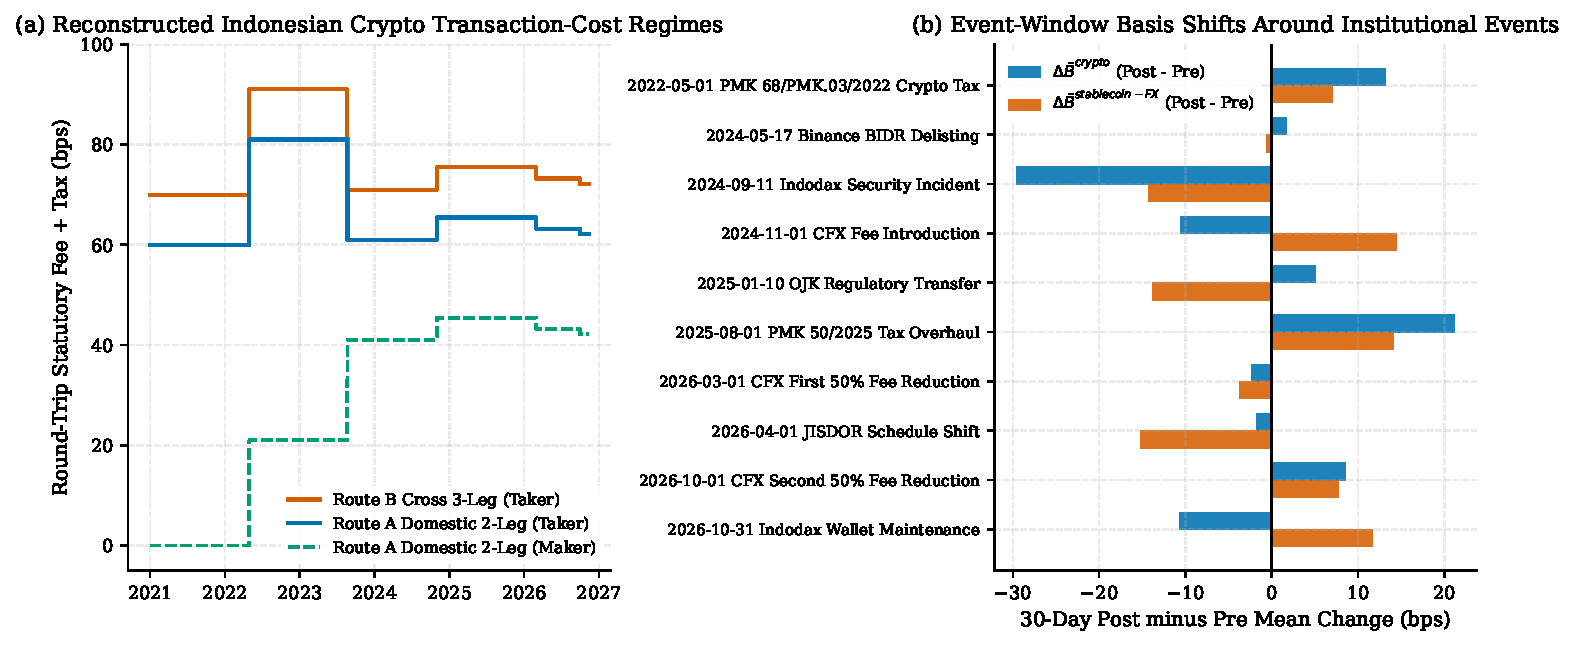
\includegraphics[width=\textwidth]{fig7_regulatory_and_costs.pdf}
  \caption{Reconstructed statutory execution cost bands across Routes A--B (Panel~a) and controlled HAC OLS $\pm 30$-day event-window basis shifts around ten institutional milestones (Panel~b; * denotes $p_{\text{Holm}} < 0.05$).}
  \label{fig:events}
\end{figure}

\section{Robustness, cross-venue validation, and falsification tests}
\label{sec:robustness}

\subsection{Timestamp alignment, JISDOR averaging window, and alternative FX benchmarks}
A common error in this literature is a fixing-to-close time mismatch (sampling 23:59 UTC crypto against an 08:15 UTC or 09:15 UTC FX benchmark). Panel~A of Table~\ref{tab:robustness} varies synchronization offsets and FX benchmarks systematically. Shifting Indodax and Binance timestamps across $\{-15\text{m}, 0\text{m}, +5\text{m}, +15\text{m}\}$ around the exact BI JISDOR fixing leaves every baseline finding invariant: mean $B_t^{total}$ moves only between $+29.48\text{ bps}$ and $+29.96\text{ bps}$ (SD $79.48$--$80.80\text{ bps}$), mean $B_t^{crypto}$ stays within $[-1.39, -0.83]\text{ bps}$, Engle--Granger $t$-statistics remain below $-4.19$ ($p \le 0.0037$), and Johansen Reinsel--Ahn trace stays tightly grouped between $150.13$ and $153.96$. Next-day JISDOR leads ($N = 1,084$) yield similar point means ($+29.40\text{ bps}$) with slightly higher total basis dispersion ($84.75\text{ bps}$). By contrast, reverting to naive 23:59 UTC crypto closing prices paired against intraday JISDOR inflates pure-crypto dispersion by $31\%$ ($35.97\text{ bps}$ versus $27.44\text{ bps}$) and flips mean $B_t^{crypto}$ sign from $-0.83\text{ bps}$ to $+2.37\text{ bps}$, which measures the size of the timestamp-mismatch bias.

\begin{table}[htbp]
\centering
\caption{Synchronization sensitivity, FX benchmark robustness, and falsification suite (BTC)}
\label{tab:robustness}
\fontsize{6.6}{7.8}\selectfont\setlength{\tabcolsep}{1.6pt}
\begingroup
\begin{tabular}{@{}>{\raggedright\arraybackslash}p{3.0cm}rrrrrrr@{}}
\toprule
\multicolumn{8}{@{}l}{\textbf{Panel A: Timestamp offset, JISDOR-window averaging, and FX benchmark sensitivity}} \\
Specification & $N$ & Mean $B^{tot}$ & SD $B^{tot}$ & Mean $B^{cry}$ & SD $B^{cry}$ & EG $t$ & Trace / Share \\
\midrule
Primary 0m JISDOR & 1,414 & 29.94 & 80.80 & -0.83 & 27.44 & -4.424 & 151.72 \\
Ex-ante $-15\text{m}$ JISDOR & 1,414 & 29.48 & 80.14 & -1.10 & 27.13 & -4.320 & 153.96 \\
Post $+5\text{m}$ JISDOR & 1,414 & 29.96 & 80.43 & -0.95 & 26.69 & -4.419 & 150.13 \\
Post $+15\text{m}$ JISDOR & 1,414 & 29.85 & 79.48 & -1.39 & 26.86 & -4.197 & 150.57 \\
Next-day JISDOR lead & 1,084 & 29.40 & 84.75 & -0.23 & 27.22 & -4.023 & 148.50 \\
23:59 UTC close mismatch & 1,414 & 31.65 & 92.03 & 2.37 & 35.97 & -4.124 & 225.32 \\
Spot FX (Yahoo) 0m & 1,251 & 40.21 & 91.20 & -0.16 & 27.01 & -4.806 & 151.09 \\
ECB FX (Frankfurter) 0m & 1,407 & 30.53 & 81.93 & -0.86 & 27.49 & -4.481 & 158.49 \\
JISDOR-win.\ VWAP (USDT only)$^\dagger$ & 1,414 & 27.06 & 82.87 & -0.83 & 27.44 & -- & 82.4\%$^\dagger$ \\
JISDOR-win.\ VWAP (all 3 legs)$^\dagger$ & 1,414 & 29.64 & 82.65 & 1.75 & 26.65 & -- & 82.8\%$^\dagger$ \\
\midrule
\multicolumn{8}{@{}l}{\textbf{Panel B: Negative controls and falsification tests}} \\
Falsification Test & $N$ & SD (bps) & EG $t$ / $F$ & $p$-val & Trace & Rej.\ 5\% & Expected Outcome \\
\midrule
Omitted FX (BTC/IDR vs.\ USDT) & 1,251 & 669.0 & -1.439 & 0.7839 & 5.81 & No & Fail cointegration \\
Wrong-FX placebo (EUR/USD) & 1,251 & 828.3 & -1.859 & 0.6006 & 6.74 & No & Fail cointegration \\
Cross-asset (BTC/IDR vs.\ XRP$\times$JISDOR) & 1,251 & 3563.3 & -2.467 & 0.2938 & 15.77 & Yes & Mixed (EG fail) \\
30-day time mismatch (BTC) & 1,221 & 2221.1 & -6.451 & $<$0.0001 & 41.87 & Yes & SD explodes \\
Calm-period break (2023-06-15) & 211 & 23.9 & 0.764 & 0.4671 & -- & No & No Chow break \\
\bottomrule
\end{tabular}\endgroup
\begin{minipage}{\textwidth}\footnotesize\vspace{3pt}
\emph{Notes:} $^\dagger$For the two JISDOR monitoring-window VWAP rows, the final column reports the resulting $\mathrm{Var}(B^{s\text{-}FX})/\mathrm{Var}(B^{total})$ share (baseline snapshot share: 83.10\%). The USDT-only VWAP row averages \texttt{USDT/IDR} over each day's exact JISDOR monitoring window while retaining snapshot BTC legs; the all-3-legs VWAP row averages \texttt{BTC/IDR}, \texttt{BTC/USDT}, and \texttt{USDT/IDR} over the monitoring window. In Panel~B, the 30-day mismatch retains algebraic cointegration because a fixed lag of an $I(1)$ price differs by a stationary 30-day return, while destroying tight parity (SD $2,221.1$ vs.\ $80.8\text{ bps}$); the cross-asset placebo fails EG ($p=0.294$) while Trace ($15.77$) marginally exceeds the $15.49$ 5\% CV.
\end{minipage}
\end{table}


A separate concern is that JISDOR is a transaction-weighted average over Bank Indonesia's intraday monitoring window (08:00--16:00 WIB on 920 days, 09:00--15:00 WIB on 432 days, and 08:00--09:45 WIB on 62 days), whereas our baseline samples \texttt{USDT/IDR} at a single five-minute bar at publication time. To check whether averaging-window mismatch inflates $\mathrm{Var}(B_t^{stablecoin\text{-}FX})$, we recompute \texttt{USDT/IDR} as the volume-weighted average (VWAP) and equal-weighted average (TWAP) of all Indodax five-minute bars inside each day's exact JISDOR monitoring window (median 97 bars per day). Matching the averaging window does not reduce stablecoin--FX dispersion: VWAP $B_t^{stablecoin\text{-}FX}$ averages $+27.89\text{ bps}$ with SD $75.22\text{ bps}$ (variance $5,658.51\text{ bps}^2$, or $104.3\%$ of the baseline snapshot variance), leaving the stablecoin--FX share of $\mathrm{Var}(B_t^{total})$ at $82.39\%$ (TWAP $82.47\%$). Volume-averaging all three legs (\texttt{BTC/IDR}, \texttt{BTC/USDT}, and \texttt{USDT/IDR}) over the exact JISDOR monitoring window gives a stablecoin--FX variance share of $82.83\%$ ($B_t^{crypto}$ SD $26.65\text{ bps}$, share $10.39\%$, covariance $6.78\%$; bottom of Table~\ref{tab:robustness}, Panel~A). The $83.1\%$ baseline share is therefore not an averaging-window artifact.

Replacing BI JISDOR with independent FX benchmarks leaves cointegration intact while revealing benchmark-specific level shifts. Pairing Indodax and Binance against ECB/Frankfurter reference rates ($N = 1,407$, SD $81.93\text{ bps}$) produces virtually identical means ($+30.53\text{ bps}$ $B_t^{total}$, $-0.86\text{ bps}$ $B_t^{crypto}$, $\text{Trace}_{RA} = 158.49$). Using continuous Yahoo Finance interbank quotes (\texttt{IDR=X}, $N = 1,251$) preserves exact pure-crypto neutrality ($-0.16\text{ bps}$ mean, $27.01\text{ bps}$ SD) and strong cointegration ($\text{Trace}_{RA} = 151.09$, $p_{boot} \leq 0.0001$), while lifting $B_t^{stablecoin\text{-}FX}$ by roughly $9.6\text{ bps}$ (to $+40.38\text{ bps}$) due to offshore non-deliverable / wholesale quote conventions relative to BI's domestic transaction-weighted JISDOR fixing.

\subsection{Calendar-day versus business-day samples and historical fee uncertainty}
Table~\ref{tab:descriptive} includes calendar-day sensitivity ($N = 2,136$) and closed-FX weekend ($N = 608$) samples to isolate forward-fill distortion. On weekends, carrying Friday's stale JISDOR rate forward inflates $B_t^{total}$ mean and variance ($+34.47\text{ bps}$ mean, SD $86.25\text{ bps}$) solely from weekend global USD/IDR gaps that cannot settle until Monday morning. Throughout those same 608 weekend dates, however, the live domestic \texttt{USDT/IDR} market keeps trading 24/7 alongside offshore crypto, holding BTC $B_t^{crypto}$ centered at $-1.70\text{ bps}$ (SD $27.84\text{ bps}$) with $98.36\%$ two-leg taker band containment. That contrast confirms that apparent weekend rupiah decoupling reflects frozen official FX clocks rather than closed crypto arbitrage.

We also test robustness to two secondary sensitivity dimensions documented in Appendices~\ref{app:provenance} and~\ref{app:details}. First, Table~\ref{tab:lag_sens} varies VECM lag orders ($k \in \{2,\dots,6\}$) and deterministic trend terms (\texttt{det\_order} $\in \{0, 1\}$): rank $r=1$ cointegration holds across all ten models ($\text{Trace}_{RA} = 51.53$ to $201.64$ versus $15.49$ and $18.40$ critical values), global BTC stays weakly exogenous ($p \in [0.191, 0.345]$), and local error-correction speeds stay within $[-0.417, -0.318]$. Second, re-evaluating dynamic cost-band containment across alternative interpretations of the partially verified May 2022--October 2023 Indodax commission cut (Section~\ref{sec:institutional}) moves total BTC $B_t^{crypto}$ containment only modestly around the $98.44\%$ baseline because Regime R2A/R2B all-in Route A taker costs stay within $61.0$--$81.0\text{ bps}$ across either $0/30$ or $10/20$ platform schedules.

\subsection{Direct multi-venue validation against Binance IDR pairs}
To verify that our primary results are not artifacts of an Indodax-specific quote anomaly, Figure~\ref{fig:robustness} compares Indodax directly against Binance's native IDR spot markets (\texttt{BTCIDR} and \texttt{USDTIDR}) across the full $N = 100,362$ five-minute overlap from November 29, 2025 at 12:30 UTC through November 12, 2026 at 23:55 UTC (the longest overlap permitted by Binance's listing date). Over those 349 days, Indodax \texttt{BTC/IDR} averages $-0.19\text{ bps}$ (SD $53.54\text{ bps}$) relative to Binance \texttt{BTC/IDR}, while Indodax \texttt{USDT/IDR} averages $-2.11\text{ bps}$ (SD $25.82\text{ bps}$) relative to Binance \texttt{USDT/IDR}. Cross-venue depth snapshots from November 13, 2026 (Table~\ref{tab:fees} and Figure~\ref{fig:robustness} right panel) explain why price leadership in domestic IDR order flow remains anchored on Indodax: executing a $\$50\text{k}$ round trip incurs $17.99\text{ bps}$ depth spread plus slippage on Indodax \texttt{BTC/IDR} versus $297.38\text{ bps}$ on Binance \texttt{BTC/IDR}, and $5.90\text{ bps}$ versus $22.20\text{ bps}$ on \texttt{USDT/IDR}.

\begin{figure}[htbp]
  \centering
  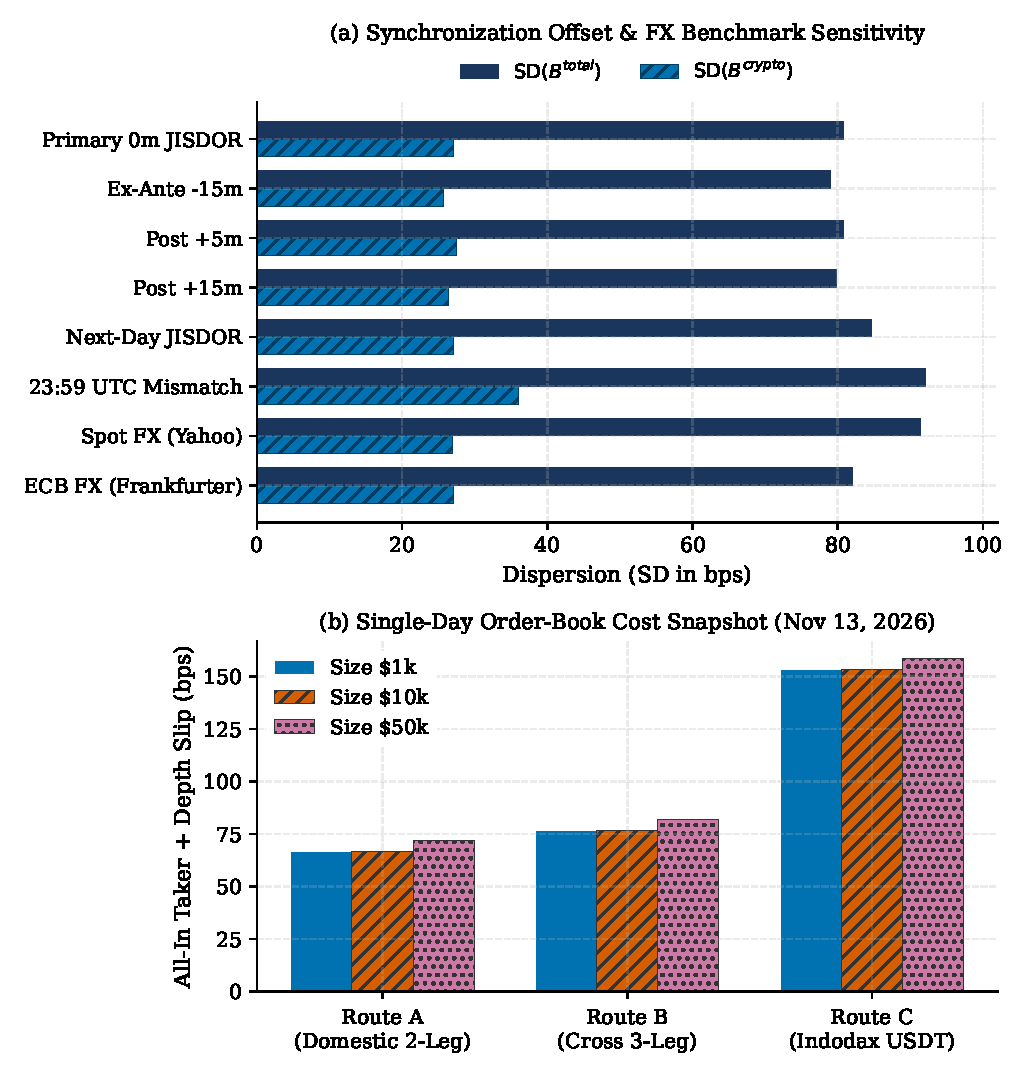
\includegraphics[width=\textwidth]{fig8_robustness_and_orderbook.pdf}
  \caption{Synchronization offset and FX benchmark sensitivity (Panel~a) and live execution cost thresholds by route and trade size from November 13, 2026 limit-order book snapshots (Panel~b).}
  \label{fig:robustness}
\end{figure}

\subsection{Negative controls and falsification suite}
Panel~B of Table~\ref{tab:robustness} reports five negative-control and placebo tests (specified before estimation in the replication code, not in an external registry) ($N = 1,251$ overlapping \texttt{IDR=X} sample for consistent cross-test comparison):
\begin{enumerate}
  \item \textbf{Omitted FX Control:} Regressing $\ln P_t^{IDR}$ on unconverted $\ln P_t^{USDT}$ inflates spread dispersion to $668.99\text{ bps}$ and fails both Engle--Granger ($t = -1.44$, $p = 0.784$) and Johansen ($\text{Trace}_{RA} = 5.81$) cointegration.
  \item \textbf{Wrong-Currency Placebo (\texttt{EUR/USD}):} Substituting euro-dollar FX rates fails to absorb long-run IDR depreciation, blowing spread SD up to $828.32\text{ bps}$ with no cointegration ($t = -1.86$, $p = 0.601$; $\text{Trace}_{RA} = 6.74$).
  \item \textbf{Cross-Asset Placebo (\texttt{BTC/IDR} vs.\ JISDOR-Converted \texttt{XRP/USDT}):} Pairing domestic bitcoin against FX-converted global ripple explodes spread dispersion to $3,563.32\text{ bps}$ ($44\times$ baseline) and fails Engle--Granger cointegration ($t = -2.47$, $p = 0.294$), although bivariate trace sits just above the $5\%$ asymptotic boundary ($15.77$ versus $15.49$) due to shared macro crypto trends over 2021--2026.
  \item \textbf{Deliberate 30-Day Timestamp Mismatch:} Lagging global crypto quotes by 30 calendar days destroys parity completely, inflating spread dispersion to $2,221.11\text{ bps}$ (versus $80.80\text{ bps}$ synchronized) because one-month asset drift overwhelms cross-market arbitrage.
  \item \textbf{Calm Subsample Placebo Break (June 15, 2023):} Testing a Chow structural-break statistic on $B_t^{crypto}$ during the calm 2023 regulatory plateau ($n = 211$) yields $F = 0.764$ ($p = 0.467$), finding no spurious structural break where none occurred.
\end{enumerate}
Collectively, the robustness and falsification checks confirm that documented cointegration, zero-mean pure crypto parity, and dynamic cost containment depend strictly on economically valid currency conversion and genuine intraday time synchronization.

\section{Discussion, methodological caveats, and policy implications}
\label{sec:discussion}

\subsection{Why apparent Indonesian bitcoin segmentation reflects conversion frictions}
Studies comparing rupiah-quoted bitcoin directly against global tether prices often report slow adjustment or persistent premia and infer that domestic capital controls or retail biases isolate local crypto order books \citep{maulana2026segmentasi,makarov2020trading}. Separating currency and stablecoin pricing with synchronized five-minute venue-specific observations tells a narrower story: the pure crypto leg on Indodax behaves like an integrated satellite book bounded by statutory trading costs. Mean BTC pure-crypto deviation is $-0.83\text{ bps}$ ($95\%$ CI $[-2.26, +0.60]\text{ bps}$), $98.44\%$ of business-day observations sit within the dynamic domestic two-leg taker fee and tax band, and the local \texttt{USDT/IDR}--JISDOR stablecoin--FX wedge accounts for $83.10\%$ of total basis variance (or $82.39\%$ when volume-averaged over JISDOR's monitoring window).

\subsection{Economic constraints on arbitraging the stablecoin--FX basis}
Why does $B_t^{stablecoin\text{-}FX}$ average $+30.77\text{ bps}$ (SD $73.66\text{ bps}$, 2021--2026) instead of collapsing toward zero? Unlike Route A and Route B crypto legs, arbitraging the \texttt{USDT/IDR}--JISDOR wedge is not a symmetric on-exchange loop. Buying USDT abroad at wholesale USD parity and selling \texttt{USDT/IDR} locally requires cross-border wire settlement, Indonesian banking intermediation, foreign-exchange spread conversion away from the mid-market JISDOR fixing, domestic rupiah settlement delays, regulatory reporting compliance under OJK and Bank Indonesia FX monitoring, and seller final PPh 22 taxes ($21\text{ bps}$ under PMK 50/2025 plus platform and CFX charges). Even when the stablecoin--FX basis drops negative during onshore USDT liquidity surges (as seen prior to October 2026 in event windows), reversing the trade into physical USD interbank balances faces settlement friction and capital-transfer costs. Consequently, $B_t^{stablecoin\text{-}FX}$ reflects fiat-rail conversion friction and onshore stablecoin demand fluctuations rather than costless unexploited profit \citep{lyons2023stablecoins,lee2022kimchi}.

\subsection{Residual verification gaps and methodological limits}
Four empirical limitations should be weighed when interpreting these estimates:
\begin{enumerate}
  \item \textbf{Partial historical verification of mid-sample Indodax fee cuts:} While pre-2022 ($0/30\text{ bps}$) and late-2024 through November 2026 schedules (including the exact five-decimal October 2026 Pro rates) are backed by primary exchange disclosures and tax statutes, day-by-day historical Pro maker/taker tiers on Indodax USDT pairs between May 2022 and October 2023 remain partially documented publicly (\texttt{PARTIALLY\_VERIFIED} in Table~\ref{tab:fees}). Containment rates inside dynamic cost bands across 2022--2023 therefore depend slightly on whether $0/30$ or $10/20$ platform commissions applied to a specific user tier.
  \item \textbf{Single multi-year domestic venue for IDR time series:} Although we tested public APIs on Tokocrypto, Pintu, and Reku, none provided downloadable multi-year historical OHLCV series comparable to Indodax. Our cross-venue comparison against Binance's direct IDR pairs (available only from November 29, 2025 onward; $N = 100,362$ five-minute bars) shows close alignment ($-0.19\text{ bps}$ mean gap on \texttt{BTC/IDR}, $-2.11\text{ bps}$ on \texttt{USDT/IDR}), yet long-horizon inferences prior to late 2025 remain Indodax-specific.
  \item \textbf{Unidentifiable daily Cholesky information shares and residual diagnostics:} Daily bivariate VECMs exhibit cross-market residual correlation $\rho_u = 0.991$ because global crypto shocks hit local and offshore books within the same 24-hour window, making Hasbrouck Information Share bounds extremely wide ($[7.1\%, 98.2\%]$). Similarly, high-frequency five-minute VECMs leave residual autocorrelation and ARCH effects ($\text{LB } p < 0.001$, $\text{ARCH } p < 0.001$), motivating Newey--West HAC standard errors throughout rather than homoskedastic likelihood standard errors alone.
  \item \textbf{Absence of historical order-book snapshots and withdrawal latency data:} Realized order-book depth slippage ($4.35$--$9.74\text{ bps}$ for $\$1\text{k}$--$\$50\text{k}$ across Routes A and B, versus $63.14$--$68.53\text{ bps}$ for Route C) is measured from live November 13, 2026 limit-order books rather than a five-year L2 replay. Historical slippage during acute volatility episodes such as March 2023 USDC de-pegging or September 2024 exchange maintenance may have been higher than November 2026 steady-state depth implies.
\end{enumerate}

\subsection{Policy implications for Bank Indonesia, OJK, and CFX}
Three concrete regulatory insights emerge. First, policymakers evaluating onshore crypto market efficiency should monitor the domestic \texttt{USDT/IDR}--JISDOR basis rather than unadjusted \texttt{BTC/IDR} premia, because domestic stablecoin conversion is the primary locus of macro-FX spillover and dollar-demand stress. Second, CFX and KKI's two-stage $50\%$ fee reductions in March and October 2026 measurably compressed statutory domestic friction by $3.33\text{ bps}$ round-trip on IDR pairs ($65.44\text{ bps} \rightarrow 62.11\text{ bps}$ taker), bringing domestic two-leg execution closer to offshore levels, whereas PMK 50/2025 ($0\%$ buyer VAT, $21\text{ bps}$ seller PPh 22) shifted tax incidence without altering symmetric round-trip statutory costs. Third, taxing onshore sell transactions at $21\text{ bps}$ alongside a $100\text{ bps}$ statutory rate on offshore venues explains why domestic liquidity stays anchored locally even as cross-venue parity persists within fee bands.

\section{Conclusion}
\label{sec:conclusion}

We examine Indonesia's rupiah cryptocurrency premium using a fixing-synchronized panel from January 2021 through November 2026 ($n = 1,414$ Bank Indonesia JISDOR business days across BTC, ETH, and XRP, paired with $616,683$ regular five-minute bars matched from $616,896$ raw Indodax and $616,683$ raw Binance bars) alongside reconstructed historical tax and exchange-fee schedules. Pre-November 2025 historical series rest on Indodax alone, complemented by 349 days of direct Binance IDR cross-checks (November 29, 2025--November 12, 2026) and a single-day November 13, 2026 order-book depth snapshot.

Four empirical findings stand out. First, once global \texttt{BTC/USDT} is converted through Indodax's synchronous \texttt{USDT/IDR} book, the pure cross-exchange crypto leg averages $-0.83\text{ bps}$ (statistically indistinguishable from zero), and $98.44\%$ of business-day deviations sit inside reconstructed dynamic domestic two-leg taker cost bands (sensitivity range $[97.52\%, 98.51\%]$ across partially verified 2022--2024 fee tiers; $97.81\%$ against the fixed $66.45\text{ bps}$ sample-average taker threshold). Second, by accounting identity, the domestic \texttt{USDT/IDR} minus JISDOR spread accounts for $83.10\%$ of total BTC basis variance ($+30.77\text{ bps}$ mean, $73.66\text{ bps}$ SD), while pure crypto deviations account for $11.53\%$ and their covariance $5.37\%$. Volume-averaging \texttt{USDT/IDR} over each day's exact Bank Indonesia JISDOR monitoring window leaves the stablecoin--FX share at $82.39\%$, so the baseline share is not an averaging-window artifact.

Third, separating Indodax \texttt{BTC/IDR}, Binance \texttt{BTC/USDT}, and Indodax \texttt{USDT/IDR} in a three-variable five-minute VECM on the regular clock-time grid ($T_{eff} = 616,677$ bars) shows that we fail to reject weak exogeneity for global Binance \texttt{BTC/USDT} ($\hat{\alpha} = +0.0011$, HAC $p = 0.418$; Hasbrouck IS $[42.6\%, 99.0\%]$), whereas Indodax \texttt{BTC/IDR} bears $80.0\%$ ($\hat{\alpha} = -0.0445$) and Indodax \texttt{USDT/IDR} bears $18.0\%$ ($\hat{\alpha} = +0.0100$) of short-run error correction, with a full-system companion half-life of $25.08$ five-minute bars (scalar $1+\beta'\alpha$ benchmark $12.09$ bars). Fourth, under controlled $\pm 30$-day HAC regressions with Holm adjustment across the 20-test event family, only the November 1, 2024 CFX/KKI fee launch survives at $5\%$ on $B_t^{stablecoin\text{-}FX}$ ($+17.37\text{ bps}$, $p_{\text{Holm}} = 0.026$, a controlled post-event association rather than a one-for-one fee pass-through), while PMK 50/2025's shift on $B_t^{crypto}$ is specification-sensitive ($+21.23\text{ bps}$, $p_{\text{Holm}} = 0.011$ unadjusted vs.\ $+17.22\text{ bps}$, $p_{\text{Holm}} = 0.275$ controlled). Measured at the JISDOR fixing, Indonesia's headline bitcoin premium is overwhelmingly a domestic stablecoin--FX spread rather than a cross-venue bitcoin price gap.


\begin{appendices}
\section{Data provenance and source exclusions}
\label{app:provenance}

\subsection{Tested venues excluded from historical time-series panels}
Alongside Bank Indonesia JISDOR, Indodax, Binance Public Data Vision, Coinbase, Kraken, Yahoo Finance, and Frankfurter (ECB), we probed public historical endpoints on three additional Indonesian-licensed trading platforms on November 13, 2026: Tokocrypto (\texttt{tokocrypto.com/open/v1/market/klines}) returned empty candle arrays, which precluded independent multi-year series construction without third-party aggregators; Pintu (\texttt{api.pintu.co.id/v2/trade/price-changes}) exposes live current-snapshot price summaries without multi-year historical candle endpoints; and Reku (\texttt{api.reku.id/v2/ticker}) exposes live snapshot tickers without open multi-year OHLCV pagination. Rather than interpolating missing venues or substituting multi-venue composite prices, we log these three domestic exchanges as tested-and-excluded. Primary empirical claims therefore characterize Indodax, Indonesia's longest-running high-volume rupiah spot exchange, relative to Binance global USDT benchmarks and Bank Indonesia JISDOR.

\section{Bootstrap validation, five-decimal tax arithmetic, and lag sensitivity}
\label{app:details}

\subsection{Five-decimal reconciliation of October 2026 Indodax Pro rates}
Under PMK No.\ 50 Tahun 2025 (effective August 1, 2025) and the October 1, 2026 CFX/KKI fee halving, published Indodax Pro rates equal:
\begin{itemize}
  \item \textbf{Buy IDR pair:} Maker $10.0\text{ bps}$ (inclusive of $11\%$ service VAT) + Buyer Asset VAT $0\text{ bps}$ + CFX/KKI IDR fee $0.555\text{ bps} = 10.555\text{ bps}$ ($0.10555\%$); Taker $= 20.0 + 0 + 0.555 = 20.555\text{ bps}$ ($0.20555\%$).
  \item \textbf{Sell IDR pair:} Maker $10.0\text{ bps}$ + Seller PPh 22 $21.0\text{ bps}$ + CFX/KKI $0.555\text{ bps} = 31.555\text{ bps}$ ($0.31555\%$); Taker $= 20.0 + 21.0 + 0.555 = 41.555\text{ bps}$ ($0.41555\%$).
  \item \textbf{Route A Round-Trip (Domestic Two-Leg):} Buying or selling across \texttt{BTC/IDR} and \texttt{USDT/IDR} gives $10.555 + 31.555 = 42.110\text{ bps}$ (maker) and $20.555 + 41.555 = 62.110\text{ bps}$ (taker).
  \item \textbf{Indodax USDT Pair:} Base $3.0/6.0\text{ bps}$ (maker/taker) + CFX USDT $1.11\text{ bps}$ + Seller PPh 22 $21.0\text{ bps} = 25.11\text{ bps}$ ($0.2511\%$) maker / $28.11\text{ bps}$ ($0.2811\%$) taker on sell orders, matching live exchange disclosures exactly.
\end{itemize}

\subsection{VAR lag order and deterministic specification sensitivity}
Table~\ref{tab:lag_sens} reports Reinsel--Ahn Johansen trace statistics and HAC VECM error-correction speeds for the synchronized BTC vs.\ JISDOR-converted global BTC system across VAR lag orders $k \in \{2,\dots,6\}$ ($k_{ar\_diff} \in \{1,\dots,5\}$) and both restricted-constant (\texttt{det\_order=0}, $H_1^*(r)$) and unrestricted-constant (\texttt{det\_order=1}, $H_1(r)$) deterministic specifications. Cointegration rank $r=1$ holds at the $1\%$ level across all ten specifications ($\text{Trace}_{RA} = 51.53$ to $201.64$ versus $15.49$ and $18.40$ critical values), while global prices remain consistently weakly exogenous ($p_{global} \in [0.191, 0.345]$) and local error-correction speeds stay between $-0.3176$ and $-0.4166$.

\begin{table}[htbp]
\centering
\caption{Johansen Cointegration and VECM Sensitivity Across Lag Orders and Deterministic Terms (BTC)}
\label{tab:lag_sens}
\fontsize{6.5}{8}\selectfont
\begingroup\setlength{\tabcolsep}{2pt}
\begin{tabular}{@{}>{\raggedright\arraybackslash}p{2.5cm}rrrrrrrr@{}}
\toprule
Det. Order & $k_{ar\_diff}$ & VAR Lag $k$ & $T_{eff}$ & Trace (RA) & 5\% CV & Reject $r=0$ & $\hat{\alpha}_{local}$ & $p_{global}$ \\
\midrule
0 (Restr.\ Const.) & 1 & 2 & 1,412 & 151.72 & 15.49 & True & $-0.3983$ & 0.2728 \\
0 (Restr.\ Const.) & 2 & 3 & 1,411 & 106.70 & 15.49 & True & $-0.4166$ & 0.1910 \\
0 (Restr.\ Const.) & 3 & 4 & 1,410 & 75.74 & 15.49 & True & $-0.3176$ & 0.3446 \\
0 (Restr.\ Const.) & 4 & 5 & 1,409 & 64.39 & 15.49 & True & $-0.3421$ & 0.2954 \\
0 (Restr.\ Const.) & 5 & 6 & 1,408 & 51.53 & 15.49 & True & $-0.3215$ & 0.2932 \\
1 (Unrestr.\ Const.) & 1 & 2 & 1,412 & 201.64 & 18.40 & True & $-0.3984$ & 0.2727 \\
1 (Unrestr.\ Const.) & 2 & 3 & 1,411 & 144.35 & 18.40 & True & $-0.4166$ & 0.1910 \\
1 (Unrestr.\ Const.) & 3 & 4 & 1,410 & 106.17 & 18.40 & True & $-0.3176$ & 0.3446 \\
1 (Unrestr.\ Const.) & 4 & 5 & 1,409 & 91.75 & 18.40 & True & $-0.3421$ & 0.2953 \\
1 (Unrestr.\ Const.) & 5 & 6 & 1,408 & 74.01 & 18.40 & True & $-0.3215$ & 0.2932 \\
\bottomrule
\end{tabular}\endgroup
\end{table}

\subsection{Direct Binance IDR spot cross-validation (November 2025--November 2026)}
Over the 349-day overlap since Binance introduced direct rupiah pairs on November 29, 2025 ($N = 100,362$ five-minute bars through November 12, 2026), Indodax \texttt{BTC/IDR} averages $-0.19\text{ bps}$ (SD $53.54\text{ bps}$) relative to Binance \texttt{BTC/IDR}, and Indodax \texttt{USDT/IDR} averages $-2.11\text{ bps}$ (SD $25.82\text{ bps}$) relative to Binance \texttt{USDT/IDR}. Because Binance \texttt{BTC/IDR} is less liquid at $\$50\text{k}$ size ($297.38\text{ bps}$ snapshot spread vs.\ $17.99\text{ bps}$ on Indodax), domestic rupiah liquidity remains heavily concentrated on Indodax even after international venue entry.

\end{appendices}

\clearpage
\section*{Declarations}
\begingroup\sloppy

\begin{itemize}
\item \textbf{Funding:} This research did not receive any specific grant from funding agencies in the public, commercial, or not-for-profit sectors.
\item \textbf{Competing interests:} The author declares that they have no known competing financial interests or personal relationships that could have appeared to influence the work reported in this paper.
\item \textbf{Data availability:} All data come from public sources (Bank Indonesia JISDOR, Indodax, Binance Public Data Vision, Coinbase, Kraken, Yahoo Finance, and Frankfurter/ECB). Raw-file hashes, cleaned panels, and replication scripts are publicly available at \texttt{https://github.com/Naresh23032003/idr-stablecoin-fx-basis}.
\item \textbf{Code availability:} All analysis code, unit tests, and table/figure generation scripts are publicly available at \texttt{https://github.com/Naresh23032003/idr-stablecoin-fx-basis}.
\item \textbf{Declaration of generative AI and AI-assisted technologies in the manuscript preparation process:} During the preparation of this work the author used Claude (Anthropic) and Gemini (Google) for language polishing, \LaTeX{} formatting, and code debugging. After using these tools, the author reviewed and edited the content as needed and takes full responsibility for the content of the publication.
\item \textbf{Author contributions (CRediT):} Naresh R: Conceptualization, Methodology, Software, Validation, Formal analysis, Investigation, Data curation, Writing -- original draft, Writing -- review \& editing, Visualization.
\item \textbf{Author ORCID:} Naresh R: \texttt{0009-0000-0735-2066} (\texttt{https://orcid.org/0009-0000-0735-2066}).
\end{itemize}
\endgroup

{\sloppy\bibliography{references}}

\end{document}
